\clearpage
% \EScomment{


\renewcommand{\contentsname}{\textsc{Appendices}}
% \renewcommand{\cfttoctitlefont}{\normalfont\large}
% \renewcommand{\cftsecfont}{\normalfont} 
% \renewcommand{\cftsecpagefont}{\normalfont}
\addcontentsline{toc}{section}{Appendices}  
\addtocontents{toc}{\protect\setcounter{tocdepth}{4}} 
\tableofcontents 


\clearpage
\section{LLM Acknowledgment}

The authors acknowledge the use of LLM for grammar corrections and for improving the clarity of the manuscript. The LLM was not used for generating original ideas, content, or experimental results. All conceptual contributions, analyses, and conclusions presented in this work are entirely from the authors.

\section{Background}

This section provides an introduction to the preliminaries of group theory. 

\subsection{Groups}
\label{sec:groups}
A group \( (G, \circ) \) consists of a non-empty set \( G \) and a binary operation \(\circ: G \times G \to G\) satisfying the following axioms:
\begin{enumerate}
    \item \textbf{Closure:} For all \( a, b \in G \), the result of the operation \( a \circ b \) is also in \( G \): \( a \circ b \in G \).
    \item \textbf{Identity Element:} There exists an element \( e \in G \) such that, for all \( a \in G \), \( a \circ e = e \circ a = a \).
    \item \textbf{Associativity:} For all \( a, b, c \in G \), \( (a \circ b) \circ c = a \circ (b \circ c) \).
    \item \textbf{Inverses:} For each \( a \in G \), there exists an element \( a^{-1} \in G \) such that \( a \circ a^{-1} = a^{-1} \circ a = e \).
\end{enumerate}

In general, not all groups are abelian. That is, the binary operation \(\circ\) does not necessarily commute:  
$
g \circ h = h \circ g,  \forall g,h \in G.
$

\subsection{Group Representations}
\label{sec:group_representations}
A group representation is a homomorphism  \(\rho: G \to GL(V)\) that assigns an \(n \times n\) matrix to each group element \(g \in G\), realizing it as a linear transformation. Representations must preserve the binary operation for all members of the group \(G\) such that:
\[
\rho(g \circ h) = \rho(g) \rho (h), \quad \forall g,h \in G.
\]

A representation \(\rho(g)\) is reducible if it can be represented as the direct sum of other representations:
\[
\rho(g) = \rho_1(g) \oplus \rho_2(g), \quad \forall g \in G.
\]

For example, a reducible \(4 \times 4\) representation of \(SU(2)\) can be decomposed into two \(2 \times 2\) sub-representations:
\[
\rho(g) =
\begin{bmatrix}
\rho_1(g) & 0 \\
0 & \rho_2(g)
\end{bmatrix}, \quad \forall g \in SU(2),
\]

where \(\rho_1(g)\) and \(\rho_2(g)\) are the following irreducible representations of \(SU(2)\):

\[
\rho_1(g) =
\begin{bmatrix}
e^{i\theta} & 0 \\
0 & e^{-i\theta}
\end{bmatrix}, \quad
\rho_2(g) =
\begin{bmatrix}
e^{i\phi} & 0 \\
0 & e^{-i\phi}
\end{bmatrix}.
\]
By contrast, irreducible representations or \textit{irreps} cannot be represented as such a direct sum. Formally, they have no non-trivial invariant subspaces \(W \subset V\) such that \(\rho(g)W \subset W, \forall g \in G\).

Representing inputs as irreps ensures equivariance by constraining each feature to transform predictably under group actions. Given \( V = \bigoplus_{i} V_i \) with irreps \( V_i \), the transformation of an input \( x \in V \) under \( g \in G \) is:  
\[
\rho(g)x = \bigoplus_{i} \rho_i(g)x_i.
\]  
Each component \( x_i \) transforms independently according to \(\rho_i\), preserving symmetry. Scalars remain invariant, while vectors rotate according to standard representations. This decomposition prevents the mixing of differently transforming features, ensuring that all subsequent operations, linear or non-linear, respect the group’s symmetry, thereby maintaining equivariance throughout the network.

% \subsection{Tensor Products}
% \label{sec:tensor_products}
% Equivariance imposes strict constraints on how neural network operations can transform input features. By Schur's lemma, given irreps \(\rho_i\) and \(\rho_j\), a linear map (e.g., weights) \(T \colon V_i \to V_j\) satisfying equivariance
% \[
% T\rho_i(g) = \rho_j(g)T, \quad \forall g \in G
% \]
% must either be the zero map or an isomorphism \(\rho_i \cong \rho_j\). This initially presents a problem for our architecture, as we are prevented from mixing features between our positions and velocities -- precisely the goal of our phase space construction.

% To circumvent this and achieve meaningful equivariance-preserving feature mixing, we employ tensor products. 
% Given two lifted embeddings \(\tilde{\mathbf{x}}, \tilde{\mathbf{v}} \in V\), each transforming according to their irreps, their tensor product is defined as
% \[
% g \cdot (\tilde{\mathbf{x}} \otimes \tilde{\mathbf{v}})
% =
% (\rho_V (g) \tilde{\mathbf{x}}) \otimes (\rho_V (g) \tilde{\mathbf{v}}).
% \]

% \[
% \tilde{\mathbf{x}} \otimes \tilde{\mathbf{v}}
% \mapsto
% (\rho_{\tilde{\mathbf{x}}} \otimes \rho_{\tilde{\mathbf{v}}})(g)(\tilde{\mathbf{x}} \otimes \tilde{\mathbf{v}})
% =
% (\rho_{\tilde{\mathbf{x}}}(g)\tilde{\mathbf{x}}) \otimes (\rho_{\tilde{\mathbf{v}}}(g) \tilde{\mathbf{v}}).
% \]
Intuitively, the tensor products capture interactions between features in a manner akin to multiplication, producing a higher-dimensional representation.
Crucially, this new representation is reducible, so we may decompose it into irreps:
\[
V \otimes V \cong \bigoplus_k V_k.
\]
It is this decomposition that allows the network to project onto individual irreps, achieving non-trivial feature mixing whilst preserving symmetry constraints.
% }

\section{Datasets}
\label{sec:dataset_construction}

We present a visualization of a sample trajectory of uracil from three datasets in Figure \ref{fig:uracil_trajectory}.

% \begin{wrapfigure}{r}{0.6\textwidth}
%     \vspace{-1em}
%     \centering
%     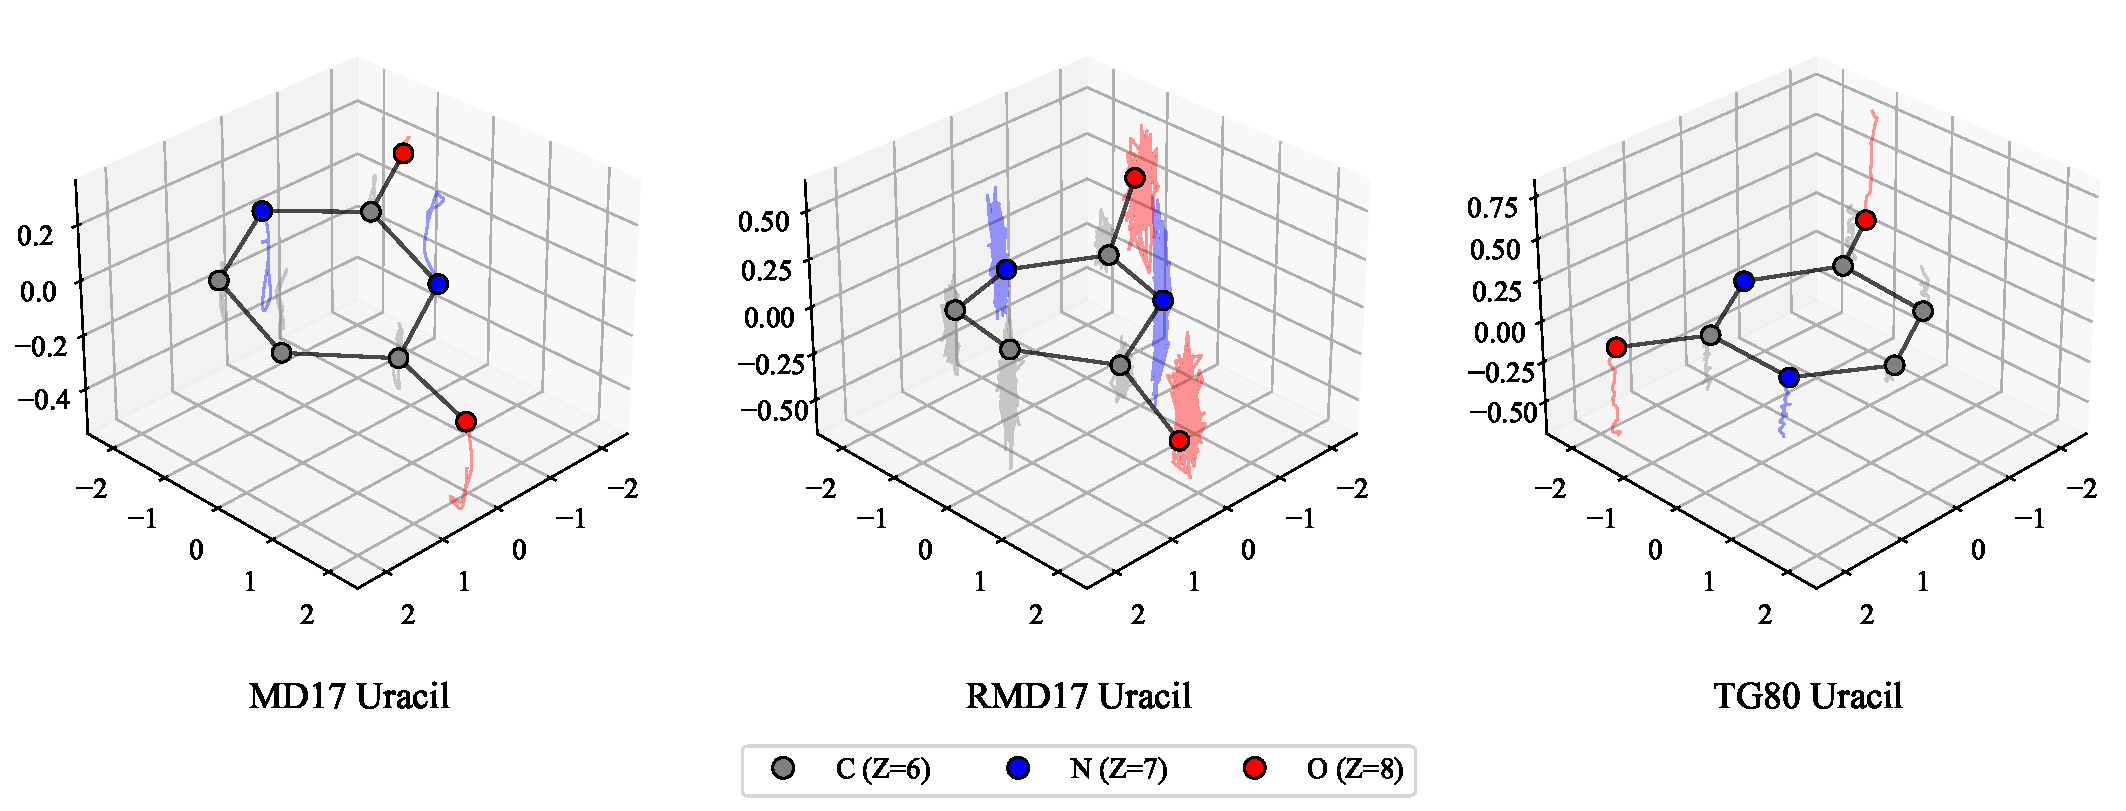
\includegraphics[width=\linewidth]{Figures/dataset/uracil_comparison.pdf}
%     \caption{3000 timesteps of uracil trajectory from MD17, RMD17, and TG80.}
%     \label{fig:uracil_trajectory}
% \end{wrapfigure}

\begin{figure}[h]
    \centering
    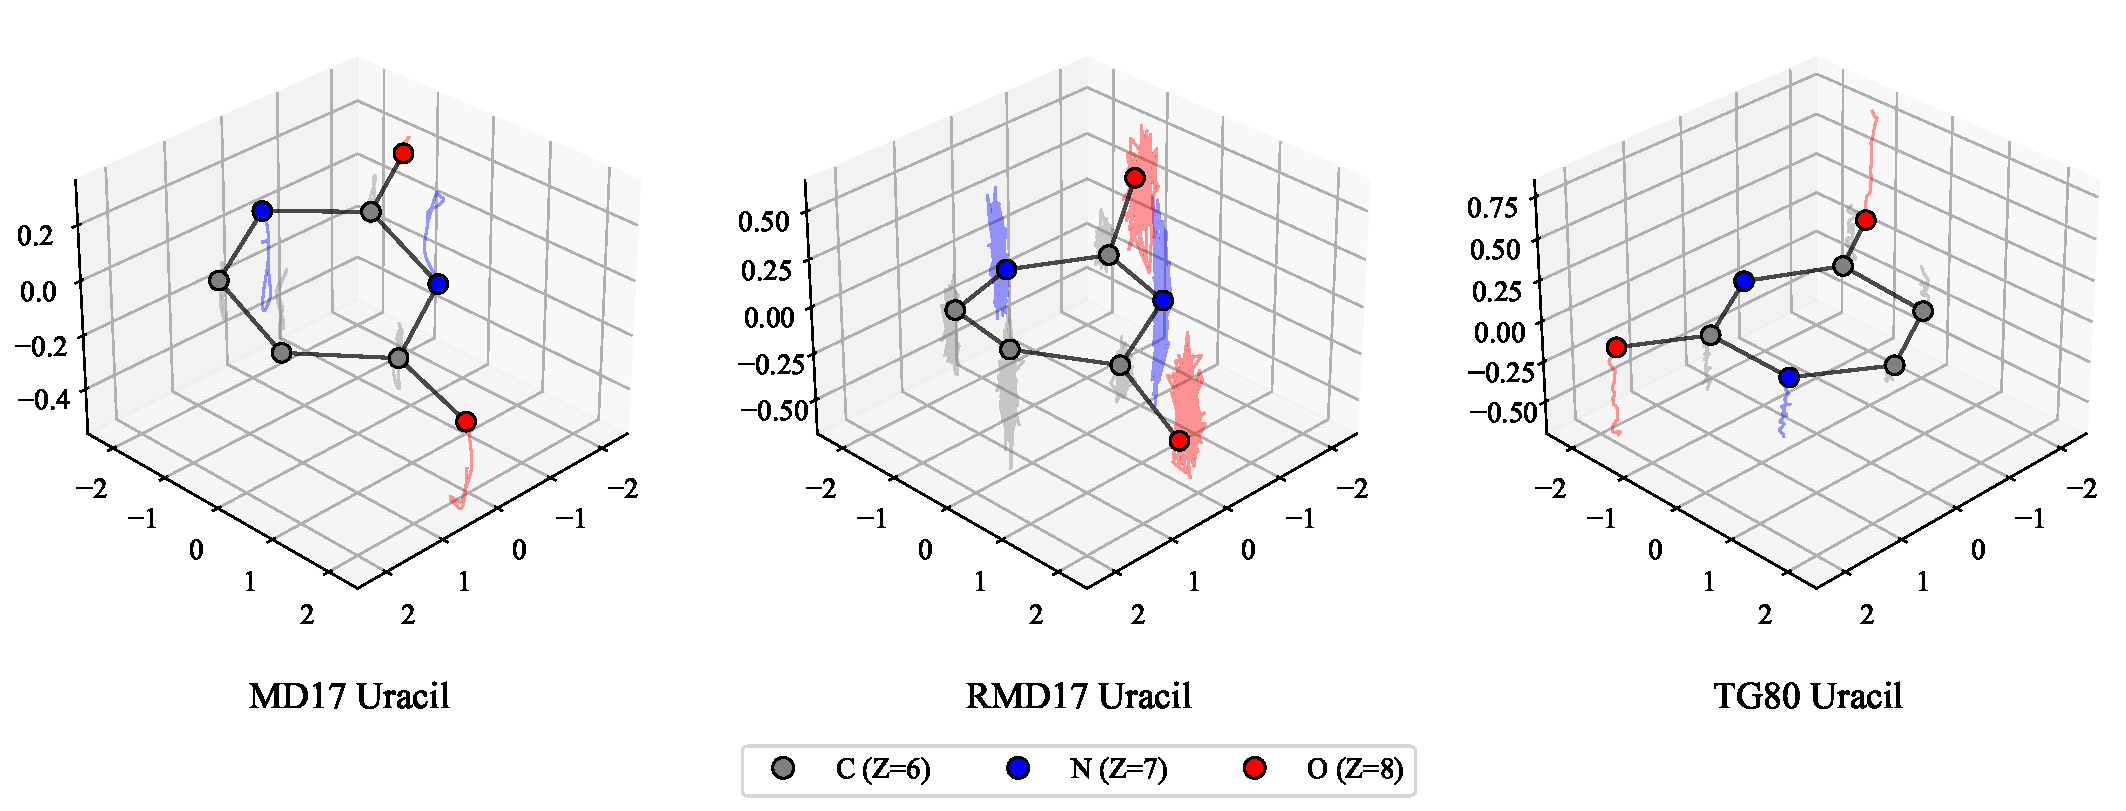
\includegraphics[width=0.8\linewidth]{Figures/dataset/uracil_comparison.pdf}
    \caption{3000 timesteps of uracil trajectory from MD17, RMD17, and TG80.}
    \label{fig:uracil_trajectory}
\end{figure}


\subsection{Licences}
\begin{table}[ht]
\centering
\caption{Dataset sources and licenses. We release TG80 under the MIT license.}
\label{tab:dataset_sources}
\rowcolors{2}{gray!10}{white}
\resizebox{\linewidth}{!}{
    \begin{tabular}{lll}
    \toprule
    \textbf{Dataset} & \textbf{Source} & \textbf{License} \\
    \midrule
    MD17            & \url{https://www.sgdml.org/} & \texttt{CC BY 4.0}\\
    RMD17           & \url{https://archive.materialscloud.org/record/2020.82} & \texttt{CC Zero V1.0 Universal} \\
    MD22           & \url{https://www.sgdml.org/} & \texttt{CC BY 4.0} \\
    TG80            & \url{https://ses.library.usyd.edu.au/handle/2123/35120} & \texttt{MIT}\\
    \bottomrule
    \end{tabular}}
\end{table}

\subsection{Model Inputs and the Dataloader}
\label{sec:dataloader}
Our compound representations follow \cite{shi_learning_2021, xu_equivariant_2024}. We model hydrogen atoms implicitly and concatenate the position and velocity norms for each node \(i\) with their respective vectors. Unlike their implementations, we avoid explicit graph construction and do not include edge labels describing atomic bond geometries.

We duplicate all frames \(\mathcal{G}^{(t)} \to \{\mathcal{G}^{(t)}\}^{P}\) during dataset initialization, producing a five-fold improvement in throughput compared to previous dataloaders in \Cref{tab:dataloader_perf}. 

\begin{table}[ht]
    \centering
    \caption{Mean time (seconds) to produce 10\,000 batches over 100 benchmark runs. Batch size = 100, 500 samples, \(\Delta t = 3000\), 500 warmup batches.}
    \label{tab:dataloader_perf}
    \begin{tabular}{lcccc}
        \toprule
         & Aspirin & Ethanol & Naphthalene & Toluene \\
         \midrule
         \gls{egno} & \(0.060{\scriptstyle \pm0.024}\) & \(0.024{\scriptstyle \pm0.016}\) & \(0.056{\scriptstyle \pm0.024}\) & \(0.039{\scriptstyle \pm0.024}\) \\
         \gls{atoms} & \(\textbf{0.005}{\scriptstyle \pm0.002}\) & \(\textbf{0.007}{\scriptstyle \pm0.002}\) & \(\textbf{0.008}{\scriptstyle \pm0.004}\) & \(\textbf{0.006}{\scriptstyle \pm0.002}\) \\
         \bottomrule
    \end{tabular}
\end{table}

\newpage
\subsection{Numerical Stability}
We evaluate the numerical stability of MD17, RMD17, and TG80. MD17 benzene exhibits substantially higher position variance in \Cref{fig:MD17_numerical_quality}, which is also partially visible in the consistent motion trails shown in \Cref{fig:MD17_trajectories}. RMD17 exhibits improved stability, with no position variance exceeding \(10\)~\AA{}\(^2\). TG80 shows the lowest median position variance of all datasets, and expectedly includes more molecules with high per-step displacement variance (due to more complex sterically hindered geometries).
\begin{figure}[H]
    \begin{subfigure}{0.49\textwidth}
        \centering
        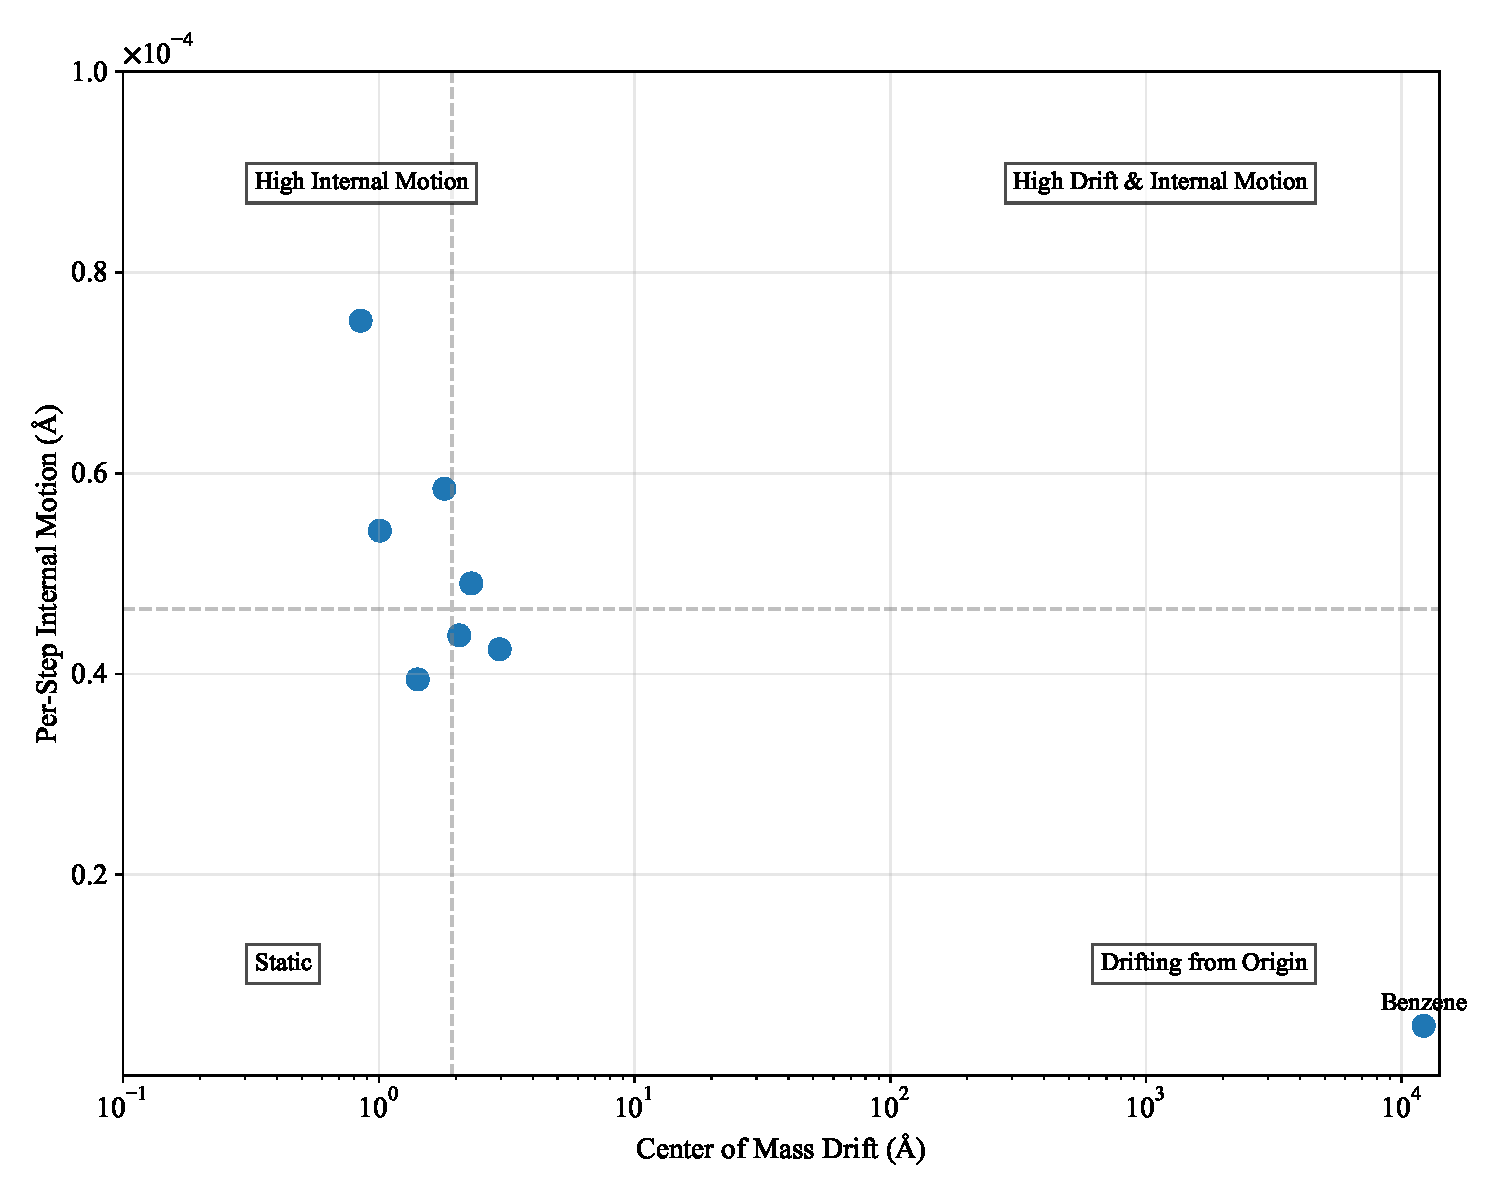
\includegraphics[width=\linewidth]{Figures/dataset/md17_molecule_behavior_comparison.pdf}
        \caption{MD17 molecules are largely consistent, except for benzene, which exhibits substantially higher position variance.}
        \label{fig:MD17_numerical_quality}
    \end{subfigure}
    \hspace{0.02\textwidth}
    \begin{subfigure}{0.49\textwidth}
        \centering
        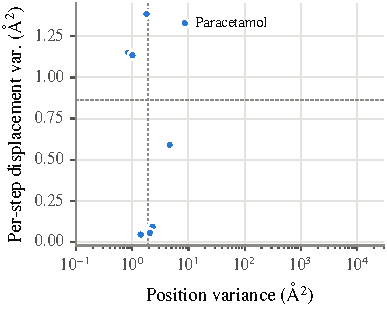
\includegraphics[width=\linewidth]{Figures/dataset/rmd17_molecule_behavior_comparison.pdf}
        \caption{RMD17 molecules are more numerically stable, supporting their use in future benchmarks.}
        \label{fig:RMD17_numerical_quality}
    \end{subfigure}
    \begin{subfigure}{\textwidth}
        \centering
        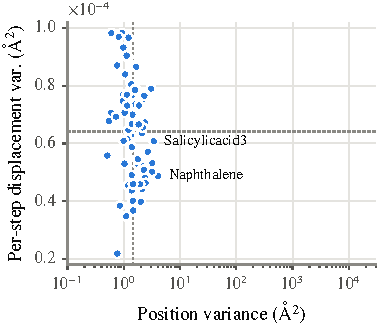
\includegraphics[width=\linewidth]{Figures/dataset/tg80_molecule_behavior_comparison.pdf}
        \caption{TG80 molecules exhibit the lowest position variance among the evaluated MD datasets.}
        \label{fig:TG80_numerical_quality}
    \end{subfigure}
    \caption{Comparison of numerical stability across MD17, RMD17, and TG80 datasets. Each point is one molecule: the x-axis is the variance of all Cartesian coordinates over the trajectory and the y-axis is the mean per-atom variance of the per-step displacement magnitude. Dashed lines denote the medians; datapoints more than two standard deviations from the median are annotated.}
    \label{fig:numerical_stability}
\end{figure}

\subsection{TG80 Generation Algorithm}
\label{sec:tg80_algorithm}
{We first recall the definition of Tanimoto \(\operatorname{T}\) similarity between two bit vectors \(X,Y\) as
\[
\operatorname{T}(X,Y) = \frac{|X \cap Y|}{|X \cup Y|},
\]
which is identical to the definition of the Jaccard similarity in this case \cite{rogers_computer_1960}.}

To generate TG80, we randomly shuffled the PubChem dataset, then iterated through all compounds until 40 were found that matched the following criteria:
\begin{wrapfigure}{r}{0.4\linewidth}
  \vspace{1em}
  \centering
  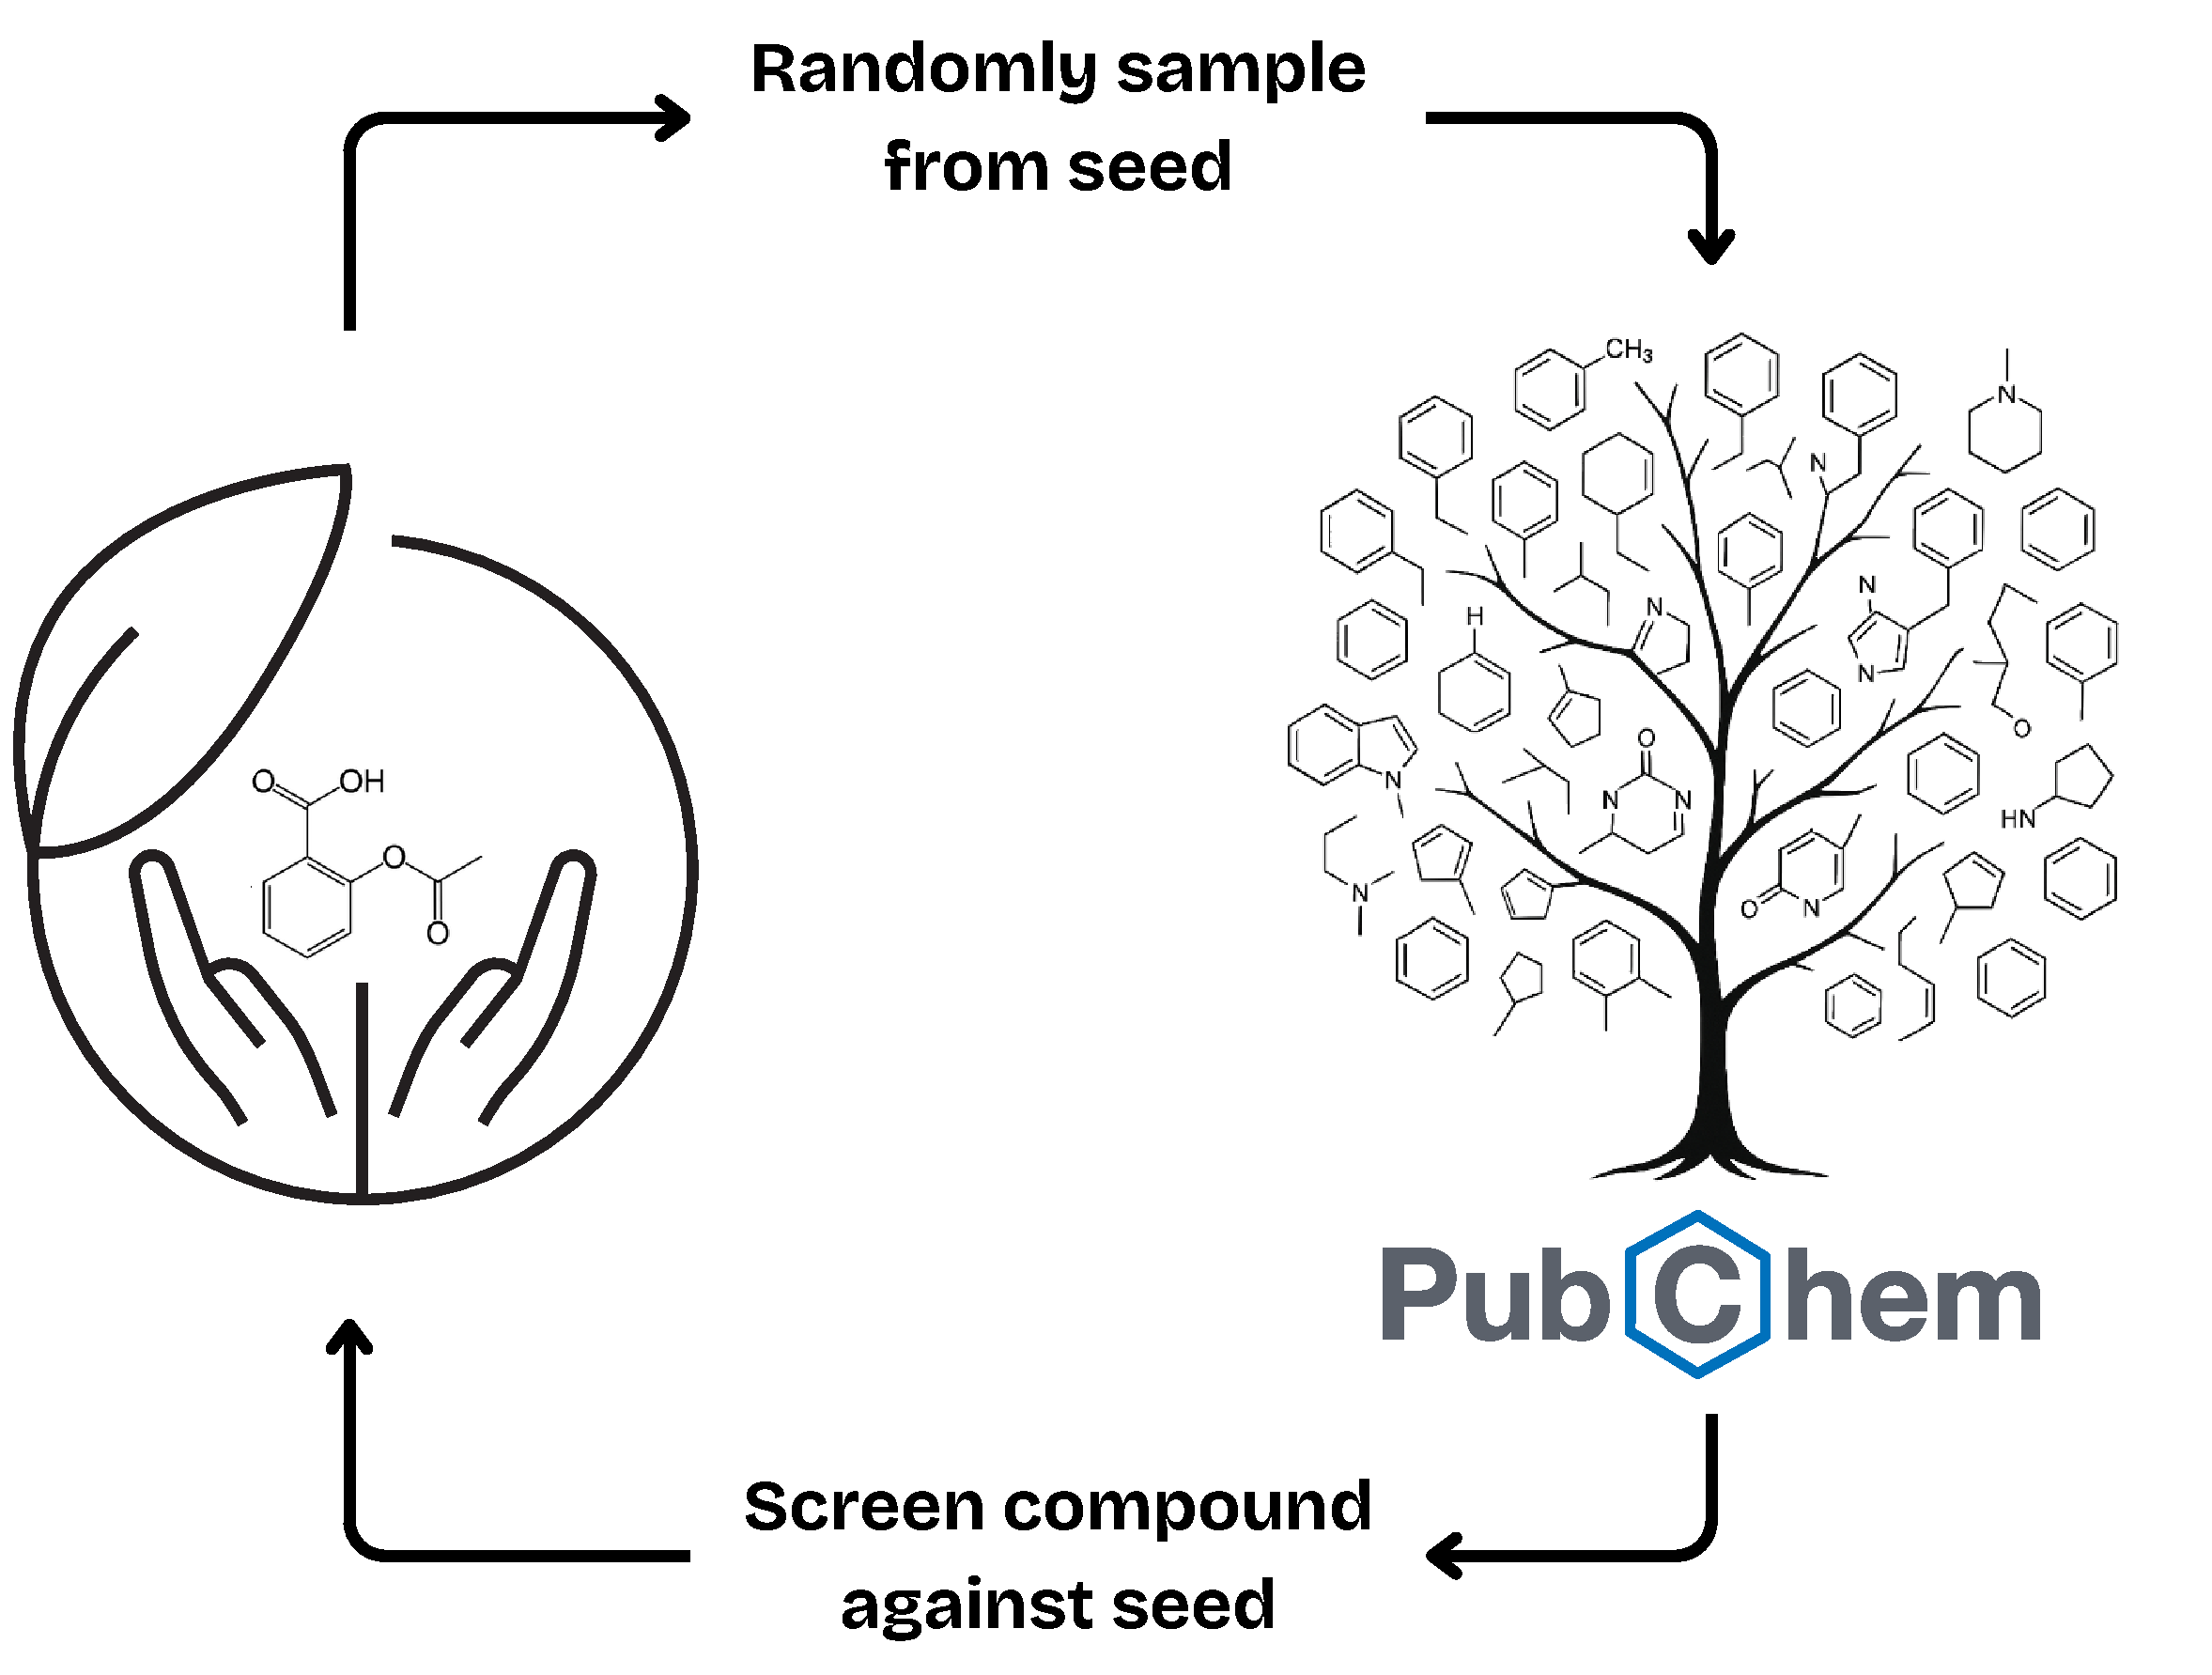
\includegraphics[width=\linewidth]{Figures/TG80.pdf}
  \caption{{Construction of TG80 from an initial seed using the PubChem database.}}
  \label{fig:dataset_construction}
  \vspace{-5em}
\end{wrapfigure}
{\begin{enumerate}
    \item \gls{smiles} encode a valid molecular structure
    \item No more heavy atoms than the corresponding seed molecule
    \item Only contain \(\{\text{C, H, O, N}\}\) atoms
    \item No more than five oxygen atoms
    \item No more than three nitrogen atoms
    \item No disconnected molecular fragments (e.g., salts)
    \item Tanimoto distance \(1-\operatorname{T}\) to at least one seed molecule between 0.875 and 0.925 (similarity between 0.075 and 0.125)
    \item Tanimoto similarity to any previously selected molecule is no more than 0.2
\end{enumerate}}
This selection procedure adds molecules that are only weakly similar to the seed set, and prevents convergence to highly similar molecules across selections. The criteria apply to the 40 selected molecules only; the 40 seed molecules include five compounds containing Cl or S (chloroform, 1,2-dichloroethane, chlorobenzene, ethanethiol and benzothiophene).

{Only 2,488 of the 173 million in the PubChem library satisfied the filtration criteria above. This low yield largely reflects the cumulative effect of criterion 8: as more molecules are added, it becomes harder to find candidates sufficiently dissimilar to all prior selections. Dataset generation code is available at \url{https://github.com/luke-a-thompson/ATOM/blob/main/data/chemical_sieve.py}.}
% \url{https://github.com/luke-a-thompson/ATOM/blob/main/data/chemical_sieve.py}

\subsection{Molecular Dynamics Simulations}
We present a complete overview of the \gls{dft} parameters used to generate MD17 \cite{chmiela_machine_2017}, RMD17 \cite{christensen_role_2020}, MD22 \cite{chmiela_accurate_2023}, and TG80.
\begin{table}[H]
    \centering
    \caption{An overview of the methodologies used to generate the \gls{md} datasets featured.}
    \label{tab:dft_techniques}
    \begin{tabular}{lccccc}
        \toprule
        & \gls{dft} Functional & Dispersion Corrections & Basis set & Timestep & Temperature \\
        \midrule
        MD17 & PBE & TS & NAO & 0.5 fs & 500K  \\
        RMD17 & PBE & None & def2-SVP & 0.5 fs & 500K  \\
        MD22 & PBE & MBD & NAO & 1.0 fs & 500K \\
        TG80 & PBE & \(\Delta 4\) & def2-SVP & 1.0 fs & 300K \\
        \bottomrule
    \end{tabular}
\end{table}

\newpage
\section{Architectural Details}
In this section, we discuss the finer architectural details of \gls{atoms} and the architectural adjustments made for our ablations.
\subsection{Fully Equivariant ATOM}
\label{sec:fully_equivariant}
To achieve the full equivariance discussed in \Cref{fig:MD17_ablation}, we employ a canonicalization network approach, which removes Euclidean gauge before learning and then reinstates it afterwards \cite{kaba_equivariance_2023}. This preserves equivariance of the whole network, even with the use of non-equivariant architectures in the trunk. This provides a controlled comparison between equivariant and non-equivariant \gls{atoms}: it enforces equivariance by construction while otherwise keeping the core architecture unchanged.

We first make data translation equivalent by centering
\begin{equation}
    \mu = \frac{1}{N}\sum_{i=1}^N x_i,
    \qquad
    \bar x_i = x_i - \mu.
\end{equation}
We then remove rotations by aligning to the second moment
\begin{equation}
    S = \tfrac{1}{N}\sum_{i=1}^N \bar x_i \bar x_i^\top
    = \sum_{k=1}^3 \lambda_k e_k e_k^\top
    \quad (\lambda_1 \ge \lambda_2 \ge \lambda_3),
\end{equation}
and choose \(e_1\) as the principal axis and orthonormalise
\begin{equation}
e_2 \leftarrow \frac{e_2 - (e_2^\top e_1)e_1}{\|e_2 - (e_2^\top e_1)e_1\|}, \qquad e_3  = e_1 \times e_2.
\end{equation}
We can then form \(Q = [e_1, e_2, e_3] \in \mathrm{SO}(3)\) and canonicalise
\begin{equation}
    \tilde x_i = (x_i-\mu)\,Q,\qquad \tilde v_i = v_i\,Q.
\end{equation}
We fix the eigenvector sign ambiguity using the chirality pseudoscalar \(c_0=\sum_{i=1}^N x_i\times v_i\) at the reference time (flip \(e_1\) to satisfy \(e_1^\top c_0\ge 0\), then adjust \(e_2,e_3\) jointly to keep right-handedness).
Let \(F\) be an arbitrary trunk acting in the canonical frame; with per-atom canonical outputs \(\hat y_i=F(\{\tilde x_j,\tilde v_j\}_{j=1}^N)_i\), we decanonicalise by
\begin{equation}
    y_i=\hat y_i\,Q^\top+\mu.
\end{equation}

This results in exact \(\mathrm{SE}(3)\)-equivariance \citep{kaba_equivariance_2023} and permits non-equivariant trunks.

On TG80 multitask learning (Cluster 1, OOD), the fully-equivariant variant reaches an S2T \gls{mse} of \(32.08{\scriptstyle \pm1.18}\times10^{-2}\), compared to \(35.47{\scriptstyle \pm0.53}\times10^{-2}\) for \gls{atoms}.

\subsection{Random-Walk Positional Encodings}
\label{sec:positional_encoding}
In the multitask case, we add row-normalized \gls{rwpe} to equip \gls{atoms} and \gls{egno} with multiscale connectivity features, enhancing their ability to distinguish non-isomorphic graphs \cite{dwivedi_graph_2022, ma_graph_2023}. We first form a \(\varepsilon\)-neighborhood graph from our pointclouds as:
\begin{equation}
    G = (V,E), \quad V = \{i\}, \quad E = \{(i,j): \|(x,y,z)_i-(x,y,z)_j\|_2 < \varepsilon\}.
\end{equation}
We set \(\varepsilon = 1.6\), as covalent bonds typically range from 1.14 \AA{} to 2.0 \AA{} in length \cite{lobato_highs_2021} and highlight that this construction does not necessitate prior knowledge of the graph structure.

Let $\mathbf{A} \in \mathbb{R}^{n \times n}$ denote the adjacency matrix of this graph, and let $\mathbf{D} = \text{diag}(\mathbf{A}\mathbf{1})$ represent its degree matrix. We construct the random walk transition matrix as \(\mathbf{M} = \mathbf{D}^{-1} \mathbf{A}\) then compute matrix powers of $\mathbf{M}$ up to a maximum walk-length $K$, defining the self-return probabilities for each node as
\begin{equation}
    p_i^{(k)} = \left(\mathbf{M}^k\right)_{ii}, \quad k = 1, \dots, K.
\end{equation}

These probabilities are collected into vectors $\mathbf{p}_i \in \mathbb{R}^{K}$ and concatenated with the phase space to form \(\hat{\mathbf{z}} = \left(\mathbf{v} \parallel \mathcal{Z} \parallel \mathbf{p}\right) \in W_\text{in}\). Here, the input feature space is redefined as \(W_\text{in} = V_\text{in} \oplus \rho_0^\text{even} \oplus \left(\rho_0^\text{even} \otimes \mathbb{R}^{K}\right)\), and the subsequent equivariant maps are modified in kind.

\subsection{Value-residual Learning}
\label{sec:value_residuals}
We employ value-residual learning wherein each transformer block receives the output of the first block via a residual connection to stabilize training and information flow through the network \cite{zhou_value_2024}. Inspired by \cite{jordan_nanogpt_2024}, we add a learned coefficient to weight this residual. Here, \(v\) denotes the current block's value output, and \(v_1\) represents the initial block's value. A learnable parameter \(\alpha\) is passed through a sigmoid to obtain the weighting coefficient:
\begin{equation}
    \lambda = \sigma(\alpha).
\end{equation}
The combined output is then given by:
\begin{equation}
    v = \lambda\,v + (1 - \lambda)\,v_1.
\end{equation}
In practice, we lock the first block's \(\lambda\) value to \(0.5\). 

% We report the learned \(\lambda\) values in \Cref{fig:lambda_values}.

% \begin{figure}[H]
%     \begin{subfigure}{0.48\textwidth}
%         \centering
%         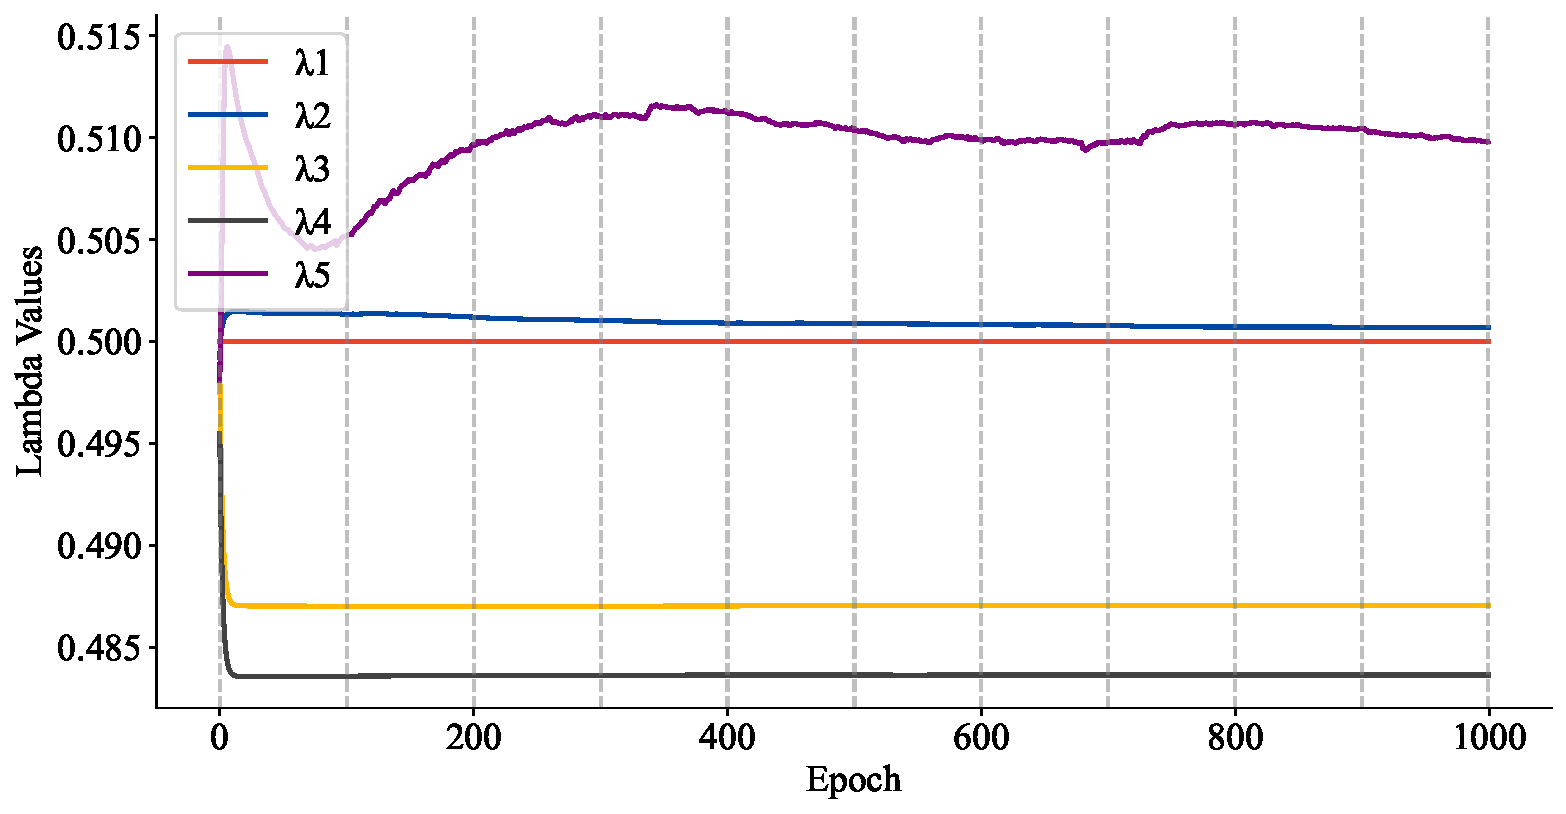
\includegraphics[width=\textwidth]{Figures/lambda_residuals/lambda_values_aspirin.pdf}
%         \caption{Aspirin}
%     \end{subfigure}
%     \hfill
%     \begin{subfigure}{0.48\textwidth}
%         \centering
%         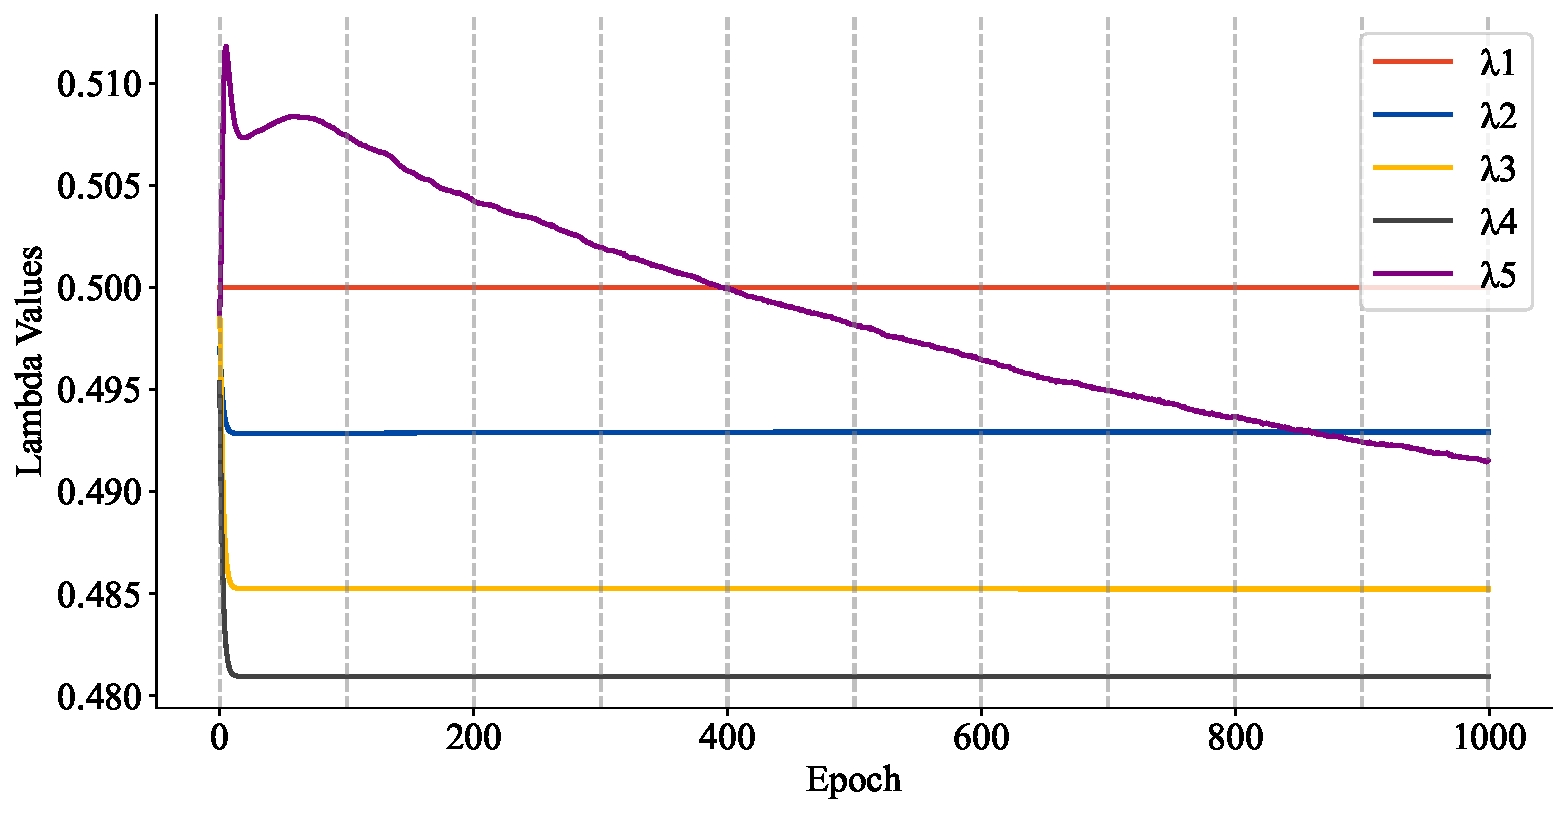
\includegraphics[width=\textwidth]{Figures/lambda_residuals/lambda_values_uracil.pdf}
%         \caption{Uracil}
%     \end{subfigure}
%     \caption{Learned value residuals for MD17 training over 1000 epochs.}
%     \label{fig:lambda_values}
% \end{figure}

% \subsection{Multi-head Output}
% \label{sec:multi_head_output}
% \EScomment{To address the diverse and class-specific dynamics observed across molecules, we employ a multi-head output layer inspired by mixture-of-experts (MoE) architectures \cite{shazeer_outrageously_2017}. Our core idea is to allow our model to dynamically select and combine several expert heads, each specializing in a distinct chemical class, thereby enhancing generalizability across the chemical space.}

% Specifically, given the set of phase space vectors \(\{ \mathbf{z}_1, \dots, \mathbf{z}_N \} = \mathbf{Z} \) of each molecule, we compute the mean pool as:
% \begin{equation}
%     \bar{\mathbf{z}} = \frac{1}{N} \sum\limits_{\mathbf{z} \in \mathbf{Z}} \mathbf{z}.
% \end{equation}
% This global vector is then fed into a softmax-normalized gating network \(\operatorname{HeadGate} \colon \mathbb{R}^d \to \mathbb{R}^{\text{n\_heads}}\), which produces a set of weights, one for each output head:
% \begin{equation}
%     \mathbf{w} = \operatorname{softmax}(\operatorname{HeadGate}(\bar{\mathbf{z}})).
% \end{equation}
% These then weight the contribution of each  \(\operatorname{Project}\) head to the final output:
% \begin{equation*}
%     \mathbf{x}^\dagger = \sum\limits_{i=1}^{\text{n\_heads}} w_i \Big( \operatorname{Project}_i(\mathbf{x}_\text{out}) \Big)
% \end{equation*}
% In the single-task learning case, a single head suffices, and the output reduces to that described in \Cref{sec:project}.

\subsection{Delta-prediction}
\label{sec:delta_prediction}
When delta-prediction is enabled, as in \Cref{fig:MD17_ablation}, we incorporate the initial positions \(\mathbf{x}\) as a residual term, reformulating the model as an operator that learns a displacement field rather than predicting absolute positions. We express this as:
\begin{equation}
    \mathbf{x}^\dagger = \operatorname{Project}(\mathbf{x}_{\text{out}}) + \mathbf{x}.
\end{equation}
Although this approach is implemented in both \gls{egnn} and \gls{egno}, we found it was disabled by default in the codebase of the latter \cite{garcia_satorras_en_2021, xu_equivariant_2024}. Based on empirical results from our ablations, \Cref{fig:MD17_ablation}, we argue there is sufficient evidence to discourage the use of delta-prediction in neural operator-based molecular dynamics simulations.



\section{Further Experiments}
\label{app:further_experiment}
We conduct further experiments on single-task and multitask learning. We consider performance under tail discretization and report results on the RMD17 dataset. For multitask learning, we report performance under random cluster assignment and S2S metrics for the experiments in \Cref{sec:multitask_learning}.

\subsection{Further Single-task Learning Experiments}

\label{app:tail_discretization}
\textbf{MD17 with tail discretization} We find the performance of both \gls{egno} and \gls{atoms} on MD17 with tail discretization remains similar to the performance under uniform discretization discussed in \cref{tab:md17_results}.

\begin{table}[H]
    \centering
    \caption{EGNO and ATOM with final frame sampling. Upper part: S2S \gls{mse}. Lower part: S2T \gls{mse}.}
    \label{tab:md17_finalframe_results}
    \resizebox{\linewidth}{!}{
    \begin{tabular}{lcccccccc}
        \toprule
         & Aspirin & Benzene & Ethanol & Malonaldehyde & Naphthalene & Salicylic & Toluene & Uracil \\
        \midrule
        \gls{egno} & \(9.69{\scriptstyle \pm0.07}\) & \(45.75{\scriptstyle \pm6.28}\) & \(4.56{\scriptstyle \pm0.00}\) & \(\mathbf{12.94}{\scriptstyle \pm0.01}\) & \(0.39{\scriptstyle \pm0.00}\) & \(0.89{\scriptstyle \pm0.01}\) & \(10.99{\scriptstyle \pm0.01}\) & \(0.58{\scriptstyle \pm0.00}\) \\
        \gls{atoms} & \(\mathbf{6.21}{\scriptstyle \pm0.13}\) & \(\mathbf{45.18}{\scriptstyle \pm1.05}\) & \(\mathbf{3.25}{\scriptstyle \pm0.03}\) & \(14.30{\scriptstyle \pm0.26}\) & \(\mathbf{0.38}{\scriptstyle \pm0.00}\) & \(\mathbf{0.81}{\scriptstyle \pm0.00}\) & \(\mathbf{5.51}{\scriptstyle \pm0.13}\) & \(\mathbf{0.54}{\scriptstyle \pm0.00}\) \\
        \midrule
        \rowcolor{gray!20} Gap & \(+35.90\%\) & \(+1.25\%\) & \(+28.78\%\) & \(-10.49\%\) & \(+4.94\%\) & \(+9.78\%\) & \(+49.87\%\) & \(+6.33\%\) \\
        \midrule
        \gls{egno} & \(9.68{\scriptstyle \pm0.07}\) & \(45.85{\scriptstyle \pm6.34}\) & \(4.56{\scriptstyle \pm0.01}\) & \(\mathbf{12.94}{\scriptstyle \pm0.01}\) & \(0.39{\scriptstyle \pm0.00}\) & \(0.89{\scriptstyle \pm0.02}\) & \(10.99{\scriptstyle \pm0.00}\) & \(0.58{\scriptstyle \pm0.00}\) \\
        \gls{atoms} & \(\mathbf{6.22}{\scriptstyle \pm0.14}\) & \(\mathbf{45.16}{\scriptstyle \pm1.05}\) & \(\mathbf{3.25}{\scriptstyle \pm0.03}\) & \(14.31{\scriptstyle \pm0.25}\) & \(\mathbf{0.37}{\scriptstyle \pm0.00}\) & \(\mathbf{0.81}{\scriptstyle \pm0.00}\) & \(\mathbf{5.51}{\scriptstyle \pm0.13}\) & \(\mathbf{0.54}{\scriptstyle \pm0.00}\) \\
        \midrule
        \rowcolor{gray!20} Gap & \(+35.80\%\) & \(+1.52\%\) & \(+28.66\%\) & \(-10.61\%\) & \(+4.97\%\) & \(+10.01\%\) & \(+49.91\%\) & \(+6.34\%\) \\
        \bottomrule
    \end{tabular}
    }
\end{table}


\textbf{Revised MD17 Dataset}
\label{sect:rmd17}
On RMD17, \gls{atoms} reduces the S2S \gls{mse} of \gls{egno} by 19.35\% and the S2T \gls{mse} by 19.89\% on average (\Cref{tab:rmd17_results}), with the largest reductions on toluene, ethanol and paracetamol. \gls{egno} is better only on malonaldehyde. RMD17 stores a random subsample of 100{,}000 frames from each original MD17 trajectory; we sort frames by their original index and only use start frames whose $P$ target frames (at offsets $i\Delta T/P$) are present in the subsample to within 5 frames.
\nopagebreak
\begin{table}[H]
    \centering
    \caption{\gls{mse} (\(\times 10^{-2}\)) of \gls{egno} and \gls{atoms} on RMD17 with uniform sampling. Upper part: S2S \gls{mse}. Lower part: S2T \gls{mse}. Gap is the relative reduction of \gls{atoms} versus \gls{egno}; the last column is the mean gap.}
    \label{tab:rmd17_results}
    \resizebox{\linewidth}{!}{
    \begin{tabular}{lccccccccc}
        \toprule
         & Azobenzene & Ethanol & Malonaldehyde & Naphthalene & Paracetamol & Salicylic & Toluene & Uracil & Mean \\
        \midrule
        \gls{egno} & \(7.33{\scriptstyle \pm0.06}\) & \(4.80{\scriptstyle \pm0.02}\) & \(\mathbf{13.06}{\scriptstyle \pm0.05}\) & \(0.49{\scriptstyle \pm0.00}\) & \(17.13{\scriptstyle \pm0.55}\) & \(0.90{\scriptstyle \pm0.01}\) & \(11.04{\scriptstyle \pm0.35}\) & \(0.62{\scriptstyle \pm0.00}\) & -- \\
        \gls{atoms} & \(\mathbf{6.61}{\scriptstyle \pm0.12}\) & \(\mathbf{3.29}{\scriptstyle \pm0.03}\) & \(13.63{\scriptstyle \pm0.07}\) & \(\mathbf{0.37}{\scriptstyle \pm0.01}\) & \(\mathbf{12.24}{\scriptstyle \pm0.15}\) & \(\mathbf{0.81}{\scriptstyle \pm0.01}\) & \(\mathbf{6.27}{\scriptstyle \pm0.06}\) & \(\mathbf{0.54}{\scriptstyle \pm0.01}\) & -- \\
        \midrule
        \rowcolor{gray!20} Gap & \(+9.88\%\) & \(+31.41\%\) & \(-4.35\%\) & \(+23.91\%\) & \(+28.56\%\) & \(+10.18\%\) & \(+43.19\%\) & \(+11.98\%\) & \(\mathbf{+19.35\%}\) \\
        \midrule
        \gls{egno} & \(6.46{\scriptstyle \pm0.05}\) & \(3.42{\scriptstyle \pm0.02}\) & \(\mathbf{11.32}{\scriptstyle \pm0.02}\) & \(0.43{\scriptstyle \pm0.01}\) & \(13.02{\scriptstyle \pm0.29}\) & \(0.93{\scriptstyle \pm0.02}\) & \(4.85{\scriptstyle \pm0.15}\) & \(0.61{\scriptstyle \pm0.01}\) & -- \\
        \gls{atoms} & \(\mathbf{5.60}{\scriptstyle \pm0.16}\) & \(\mathbf{2.51}{\scriptstyle \pm0.00}\) & \(11.61{\scriptstyle \pm0.06}\) & \(\mathbf{0.36}{\scriptstyle \pm0.00}\) & \(\mathbf{9.98}{\scriptstyle \pm0.07}\) & \(\mathbf{0.67}{\scriptstyle \pm0.01}\) & \(\mathbf{2.87}{\scriptstyle \pm0.03}\) & \(\mathbf{0.52}{\scriptstyle \pm0.01}\) & -- \\
        \midrule
        \rowcolor{gray!20} Gap & \(+13.30\%\) & \(+26.80\%\) & \(-2.54\%\) & \(+15.70\%\) & \(+23.37\%\) & \(+27.61\%\) & \(+40.81\%\) & \(+14.11\%\) & \(\mathbf{+19.89\%}\) \\
        \bottomrule
    \end{tabular}
    }
\end{table}
% \begin{table}[H]
%     \centering
%     \caption{\gls{mse} (\(\times 10^{-2}\)) on RMD17. Upper part: S2S \gls{mse}. Lower part: S2T \gls{mse}}
%     \label{tab:rmd17_results_old}
%     \resizebox{\linewidth}{!}{
%     \begin{tabular}{lccccccccc}
%         \toprule
%         & Azobenzene & Ethanol & Malonaldehyde & Naphthalene & Paracetamol & Salicylic & Toluene & Uracil & Mean \% \\
%         \midrule
%         \gls{egno} & \(10.82{\scriptstyle \pm0.05}\) & \(28.27{\scriptstyle \pm0.16}\) & \(49.25{\scriptstyle \pm0.10}\) & \(1.85{\scriptstyle \pm0.01}\) & \(28.90{\scriptstyle \pm0.20}\) & \(1.26{\scriptstyle \pm0.01}\) & \(28.44{\scriptstyle \pm0.18}\) & \(0.98{\scriptstyle \pm0.01}\) \\
%         \gls{atoms} & \(\mathbf{8.36}{\scriptstyle \pm0.01}\) & \(\mathbf{23.81}{\scriptstyle \pm1.29}\) & \(\mathbf{39.87}{\scriptstyle \pm0.53}\) & \(\mathbf{1.42}{\scriptstyle \pm0.01}\) & \(\mathbf{28.74}{\scriptstyle \pm0.33}\) & \(\mathbf{1.09}{\scriptstyle \pm0.01}\) & \(28.48{\scriptstyle \pm0.02}\) & \(\mathbf{0.89}{\scriptstyle \pm0.01}\) \\
%         \midrule
%         \rowcolor{gray!20} Gap (\%) & \(22.74\%\) & \(15.78\%\) & \(19.05\%\) & \(23.24\%\) & \(0.55\%\) & \(13.49\%\) & \(-0.14\%\) & \(9.18\%\) & \(\mathbf{12.99\%}\) \\
        
%         \midrule
%         \gls{egno} & \(10.75{\scriptstyle \pm0.05}\) & \(28.19{\scriptstyle \pm0.16}\) & \(48.78{\scriptstyle \pm0.10}\) & \(1.80{\scriptstyle \pm0.01}\) & \(\mathbf{28.29}{\scriptstyle \pm0.20}\) & \(1.25{\scriptstyle \pm0.01}\) & \(28.37{\scriptstyle \pm0.18}\) & \(0.98{\scriptstyle \pm0.01}\) \\
%         \gls{atoms} & \(\mathbf{8.61}{\scriptstyle \pm0.01}\) & \(\mathbf{23.48}{\scriptstyle \pm 
%         0.14}\) & \(\mathbf{40.36}{\scriptstyle \pm0.33}\) & \(\mathbf{1.41}{\scriptstyle \pm0.01}\) & \(28.79{\scriptstyle \pm0.33}\) & \(\mathbf{1.08}{\scriptstyle \pm0.01}\) & \(28.45{\scriptstyle \pm0.071}\) & \(\mathbf{0.89}{\scriptstyle \pm0.01}\) \\
%         \midrule
%         \rowcolor{gray!20} Gap (\%) & \(19.91\%\) & \(16.71\%\) & \(17.26\%\) & \(21.67\%\) & \(-1.77\%\) & \(13.60\%\) & \(-0.28\%\) & \(9.18\%\) & \(\mathbf{12.04\%}\) \\
%         \bottomrule
%     \end{tabular}
%     }
% \end{table}

\subsection{Further Multitask Learning Experiments}

\label{sect:random_split}
\textbf{Random-split cross-validation on TG80.} For completeness, we report multitask results under compound-level random cross-validation, where compounds are randomly assigned to the train, validation, and test sets. Relative to the more challenging out-of-domain (UMAP-based) split in \Cref{tab:tg80_umap}, \gls{egno} is comparatively stronger; nevertheless, \gls{atoms} maintains a consistent lead across folds, with mean improvements of 25.10\% on S2S and 25.07\% on S2T.

\begin{table}[H]
  \centering
  \caption{S2S \gls{mse} \((\times10^{-2})\) on TG80 across five random cluster assignments.}
  \resizebox{\linewidth}{!}{%
  \begin{tabular}{llccccc}
    \toprule
     &  & \textbf{Cluster 1} & \textbf{Cluster 2} & \textbf{Cluster 3} & \textbf{Cluster 4} & \textbf{Cluster 5} \\
     \midrule
    \multirow{2}{*}{OOD}
       & \gls{egno} & \(71.83{\scriptstyle \pm0.00}\) & \(76.92{\scriptstyle \pm0.00}\) & \(68.99{\scriptstyle \pm0.00}\) & \(101.27{\scriptstyle \pm0.00}\) & \(83.20{\scriptstyle \pm0.00}\) \\
       & \gls{atoms} & \(\mathbf{56.88}{\scriptstyle \pm0.88}\) & \(\mathbf{59.34}{\scriptstyle \pm0.98}\) & \(\mathbf{54.78}{\scriptstyle \pm1.54}\) & \(\mathbf{67.23}{\scriptstyle \pm6.88}\) & \(\mathbf{60.22}{\scriptstyle \pm2.19}\) \\
      \cmidrule(lr){2-7}
      \rowcolor{gray!20} & Gap & \(+20.81\%\) & \(+22.85\%\) & \(+20.60\%\) & \(+33.62\%\) & \(+27.63\%\) \\
    \bottomrule
  \end{tabular}
  }
  \label{tab:tg80_random_s2s}
\end{table}

\begin{table}[H]
  \centering
  \caption{S2T \gls{mse} \((\times10^{-2})\) on TG80 across five random cluster assignments.}
  \resizebox{\linewidth}{!}{%
  \begin{tabular}{llccccc}
    \toprule
     &  & \textbf{Cluster 1} & \textbf{Cluster 2} & \textbf{Cluster 3} & \textbf{Cluster 4} & \textbf{Cluster 5} \\
     \midrule
    \multirow{2}{*}{OOD}
       & \gls{egno} & \(63.23{\scriptstyle \pm0.00}\) & \(64.49{\scriptstyle \pm0.00}\) & \(59.18{\scriptstyle \pm0.00}\) & \(85.87{\scriptstyle \pm0.00}\) & \(69.46{\scriptstyle \pm0.00}\) \\
       & \gls{atoms} & \(\mathbf{48.61}{\scriptstyle \pm1.89}\) & \(\mathbf{50.96}{\scriptstyle \pm1.34}\) & \(\mathbf{46.54}{\scriptstyle \pm1.36}\) & \(\mathbf{57.72}{\scriptstyle \pm7.32}\) & \(\mathbf{50.66}{\scriptstyle \pm2.14}\) \\
      \cmidrule(lr){2-7}
      \rowcolor{gray!20} & Gap & \(+23.13\%\) & \(+20.99\%\) & \(+21.37\%\) & \(+32.79\%\) & \(+27.07\%\) \\
    \bottomrule
  \end{tabular}
  }
  \label{tab:tg80_random_s2t}
\end{table}


\textbf{Multitask S2S results on TG80 under UMAP cluster cross-validation.} The S2S side of the multitask learning results follow closely from their S2T counterparts presented in \Cref{sec:multitask_learning}.
\label{app:s2s_result}

\begin{table}[H]
  \centering
  \caption{S2S \gls{mse} \((\times10^{-2})\) on TG80 across five UMAP cluster assignments. Gap is the relative reduction of \gls{atoms} versus \gls{egno}.}
  \resizebox{\linewidth}{!}{%
  \begin{tabular}{llccccc}
    \toprule
     &  & \textbf{Cluster 1} & \textbf{Cluster 2} & \textbf{Cluster 3} & \textbf{Cluster 4} & \textbf{Cluster 5} \\
     \midrule
     \multirow{3}{*}{ID}
      & \gls{egno}  & \(51.83{\scriptstyle \pm0.79}\) & \(103.99{\scriptstyle \pm0.22}\) & \(143.61{\scriptstyle \pm0.84}\) & \(154.75{\scriptstyle \pm0.60}\) & \(109.30{\scriptstyle \pm0.33}\) \\
      & \gls{atoms} & \(\mathbf{6.18}{\scriptstyle \pm0.25}\) & \(\mathbf{9.05}{\scriptstyle \pm0.35}\) & \(\mathbf{5.95}{\scriptstyle \pm0.16}\) & \(\mathbf{5.08}{\scriptstyle \pm0.45}\) & \(\mathbf{6.18}{\scriptstyle \pm0.41}\) \\
      \cmidrule(lr){2-7}
      \rowcolor{gray!20} & Gap (\%) & \(88.08\%\) & \(91.30\%\) & \(95.86\%\) & \(96.72\%\) & \(94.34\%\) \\
    \midrule
    \multirow{4}{*}{OOD}
      & \gls{egno}  & \(53.19{\scriptstyle \pm0.96}\) & \(1788.34{\scriptstyle \pm2874.88}\) & \(149.38{\scriptstyle \pm1.55}\) & \(163.23{\scriptstyle \pm0.40}\) & \(112.36{\scriptstyle \pm1.70}\) \\
      & EGNN\text{-}S & \(52.46{\scriptstyle \pm0.43}\) & \(59210.80{\scriptstyle \pm52351.92}\) & \(150.22{\scriptstyle \pm1.10}\) & \(2965.22{\scriptstyle \pm4852.19}\) & \(111.18{\scriptstyle \pm0.57}\) \\
      & EGNN\text{-}R & \(52.11{\scriptstyle \pm0.93}\) & \(116.96{\scriptstyle \pm0.68}\) & \(151.26{\scriptstyle \pm2.45}\) & \(163.20{\scriptstyle \pm0.27}\) & \(110.88{\scriptstyle \pm1.90}\) \\
      & \gls{atoms} & \(\mathbf{42.75}{\scriptstyle \pm0.31}\) & \(\mathbf{72.22}{\scriptstyle \pm5.54}\) & \(\mathbf{86.26}{\scriptstyle \pm7.00}\) & \(\mathbf{97.83}{\scriptstyle \pm7.30}\) & \(\mathbf{63.71}{\scriptstyle \pm4.79}\) \\
      \cmidrule(lr){2-7}
      \rowcolor{gray!20} & Gap (\%) & \(19.62\%\) & \(95.96\%\) & \(42.25\%\) & \(40.07\%\) & \(43.30\%\) \\
    \bottomrule
  \end{tabular}
  }
  \label{tab:tg80_umap_s2s}
\end{table}

\newpage

\begin{wraptable}{r}{0.42\textwidth}
    \centering
    \caption{\gls{mse} \((\times10^{-2})\) on full-dataset TG80 \gls{atoms} and single-task \gls{atoms}. S2S upper, S2T lower.}
    \begin{tabular}{lc}
        \toprule
        & Formic Acid \\
        \midrule
        Single-task \gls{atoms} & \textbf{26.51} \\
        All-data \gls{atoms} & 29.37 \\
        \midrule
        \rowcolor{gray!20} Gap (\%) & \(-10.79\%\) \\
        \midrule
        Single-task \gls{atoms} & \textbf{17.80} \\
        All-data \gls{atoms} & 19.92 \\
        \midrule
        \rowcolor{gray!20} Gap (\%) & \(-11.91\%\) \\
        \bottomrule
    \end{tabular}
    \label{tab:placeholder}
    \vspace{-0.5\baselineskip}
\end{wraptable}
\textbf{Multitask S2S Versus Single Task} We evaluate a multitask \gls{atoms} model trained on all available trajectories, pooling both ID and OOD clusters, against a single-task \gls{atoms} trained separately on each compound. On formic acid, the multitask model comes within 12\% of the single-task model on both S2S and S2T \gls{mse}, while also covering every other compound in TG80.

% \begin{table}[H]
%     \centering
%     \caption{\gls{mse} \((\times10^{-2})\) on full-dataset TG80 \gls{atoms} and single-task \gls{atoms}. S2S upper, S2T lower.}
%     \begin{tabular}{lc}
%         \toprule
%         & Formic Acid \\
%         \midrule
%         Single-task \gls{atoms} & 26.40 \\
%         All-data \gls{atoms} & \textbf{22.39} \\
%         \midrule
%         \rowcolor{gray!20} Gap (\%) & \(15.19\%\) \\
%         \midrule
%         Single-task \gls{atoms} & \textbf{18.10} \\
%         All-data \gls{atoms} & 18.72 \\
%         \midrule
%         \rowcolor{gray!20} Gap (\%) & \(-3.43\%\) \\
%         \bottomrule
%     \end{tabular}
%     \label{tab:placeholder}
% \end{table}

% in text

\subsection[Monte Carlo Estimation of Quasi-equivariance]{Monte Carlo Estimation of\\ Quasi-equivariance}
\label{app:quasi_equivariance_mc}
{For both the pretrained \gls{atoms} and the non-equivariant lifting variant, we estimate the quantity in \Cref{def:quasi_equivariance} by Monte Carlo, drawing \(N\) test states \(x_n\) and, for each, \(R\) rotations \(g_{n,r}\) sampled uniformly (Haar) from \(\mathrm{SO}(3)\). We approximate
\begin{equation*}
    \varepsilon \approx \frac{1}{N R} \sum_{n=1}^{N} \sum_{r=1}^{R}
    \left\|
            f\bigl(\phi(g_{n,r})(x_n)\bigr)
            - \rho(g_{n,r})\bigl(f(x_n)\bigr)
    \right\|_2 ,
\end{equation*}
where the norm is taken over the Cartesian coordinates of each predicted atom position and the result is averaged over atoms and predicted timesteps.
We report our estimates of \(\varepsilon\) for various \gls{atoms} models trained on MD17 single task learning in \Cref{tab:equivariance_defect}. \gls{atoms} shows a lower equivariance defect than the non-equivariant variant on aspirin, malonaldehyde and toluene, with the largest reduction on toluene (\(2.2\times\)); on ethanol, naphthalene, salicylic acid and uracil the non-equivariant variant has the lower defect.
}

\begin{table}[H]
%— Top: Full‐width big table —
\centering
\caption{Estimates of the equivariance defect \(\varepsilon\) \((\times10^{-2}\)~\AA{}) via Monte Carlo over 20 Haar-random rotations and 10 test batches with 2SD intervals.}
\label{tab:equivariance_defect}
\resizebox{\linewidth}{!}{%
    \begin{tabular}{lccccccc}
        \toprule
         & Aspirin & Ethanol & Malonaldehyde & Naphthalene & Salicylic & Toluene & Uracil \\
        \midrule 
        Non-equivariant \gls{atoms} & \(137.72{\scriptstyle \pm85.15}\) & \(\mathbf{35.48}{\scriptstyle \pm18.91}\) & \(57.55{\scriptstyle \pm32.70}\) & \(\mathbf{88.66}{\scriptstyle \pm41.67}\) & \(\mathbf{119.18}{\scriptstyle \pm64.44}\) & \(3750.90{\scriptstyle \pm3815.93}\) & \(\mathbf{108.73}{\scriptstyle \pm78.73}\) \\

        \textbf{\gls{atoms}} & \(\mathbf{130.09}{\scriptstyle \pm95.67}\) & \(37.47{\scriptstyle \pm22.68}\) & \(\mathbf{52.25}{\scriptstyle \pm31.70}\) & \(204.68{\scriptstyle \pm174.68}\) & \(259.44{\scriptstyle \pm188.28}\) & \(\mathbf{1710.83}{\scriptstyle \pm1868.94}\) & \(229.57{\scriptstyle \pm228.08}\) \\
        \bottomrule
    \end{tabular}
}
\end{table}



% \subsection{Explicit Hydrogen Representation}
% We hypothesized that our model's underperformance relative to \gls{egno} in predicting malonaldehyde was due to the omission of explicit hydrogens, which limits its ability to capture electron delocalization effects involving hydroxyl hydrogens. We tested two explicit hydrogen methods: 
% \begin{enumerate}
%     \item Including all hydrogens with gradients computed for all atoms during training
%     \item Including all hydrogens but computing gradients only for heavy atoms
% \end{enumerate}

% Contrary to conventional \gls{md} practice, neither method improved heavy-atom test loss.

% \begin{table}[H]
%     \centering
%     \caption{\gls{atoms} MD17 S2T MSE with implicit hydrogens (\gls{atoms} baseline) and two explicit hydrogen approaches.}
%     \label{tab:explicit_hydrogens}
%     \begin{tabular}{lcc}
%         \toprule
%         & Aspirin & Malonaldehyde \\
%         \midrule
%         Explicit hydrogens 1 & \(7.48{\scriptstyle \pm0.11}\) & \(15.15{\scriptstyle \pm0.22}\) \\
%         Explicit hydrogens 2 & \(6.96{\scriptstyle \pm0.20}\) & \(13.52{\scriptstyle \pm0.10}\)\\
%         Implicit hydrogens & \(6.52{\scriptstyle \pm0.08}\) & \(13.51{\scriptstyle \pm0.10}\) \\
%         \bottomrule
%     \end{tabular}
% \end{table}

% \subsection{Varying T-RoPE Base}
% We experimented with several \gls{trope} bases, but found no difference in performance at either \(P=8\) pr \(P=32\). Our results are available in \Cref{tab:trope_bases}.
% \begin{table}[H]
%     \centering
%     \caption{S2T \gls{mse} across varying \gls{trope} bases and \(P\).}
%     \label{tab:trope_bases}
%     \begin{tabular}{lcc}
%         \toprule
%         Base & \(P=8\) & \(P=16\) \\
%         \midrule
%         100 & \(5.41{\scriptstyle \pm0.13}\) & \(5.41{\scriptstyle \pm0.13}\) \\
%         1000 & \(5.61{\scriptstyle \pm0.04}\) & \(5.38{\scriptstyle \pm0.31}\) \\
%         10\,000 & \(5.57{\scriptstyle \pm0.04}\) & \(5.39{\scriptstyle \pm0.05}\) \\
%         100\,000 & \(5.69{\scriptstyle \pm0.13}\) & \(5.52{\scriptstyle \pm0.26}\) \\
%         \bottomrule
%     \end{tabular}
% \end{table}

\section{Experimental Details}
\label{sect:details}

\subsection{Software and Hardware Details}
All experiments were conducted using Python 3.12, NumPy 2.2.1 \cite{harris_array_2020}, PyTorch 2.5.1 \cite{paszke_pytorch_2019}, e3nn 0.5.6 \cite{geiger_e3nn_2022} and PyTorch Optimizer 3.5.0 \cite{kim_pytorch_optimizer_2021}. We use RDKit 2024.9.6 \cite{greg_landrum_rdkitrdkit_2025} and PubChemPy 1.0.4 to construct TG80. All single-task training was performed on an NVIDIA RTX 5080 (16 GB) with CUDA 12.4, running on Ubuntu 24.04. {We use Ase 3.26.0 \cite{larsen_atomic_2017} and MACE-Torch 0.3.14 \cite{kovacs_mace-off_2025} in the experiments of \Cref{app:inference_times}.}

\subsection{Training Times and Compute Requirements}
\label{sec:model_compute_time}
\textbf{Single-task training time} We roughly wall-clock normalised our \gls{atoms} and \gls{egno} parameter counts, resulting in respective learnable parameter counts of 910\,320 and 335\,770.

\begin{table}[H]
    \centering
    \caption{Compute cost of single-task training on all RMD17 molecules over 1000 epochs. Both \gls{atoms} (910\,320 params) and \gls{egno} (335\,770 params) are under \texttt{torch.compile} on a Titan V. Total FLOPS is wall-clock time multiplied by the peak FP32 throughput of the GPU.}
    \label{tab:md17_compute_cost}
    \resizebox{\linewidth}{!}{%
    \begin{tabular}{llcccccccc}
            \toprule
            Model & Metric & Azobenzene & Ethanol & Malonaldehyde & Naphthalene & Paracetamol & Salicylic & Toluene & Uracil \\
            \midrule
            \multirow{3}{*}{\gls{egno}}
             & Time (mins) & \(4.09\pm\scriptstyle{0.15}\) & \(3.62\pm\scriptstyle{0.42}\) & \(3.65\pm\scriptstyle{0.01}\) & \(5.01\pm\scriptstyle{0.02}\) & \(9.02\pm\scriptstyle{1.22}\) & \(5.16\pm\scriptstyle{0.03}\) & \(3.93\pm\scriptstyle{0.02}\) & \(4.35\pm\scriptstyle{0.04}\) \\
             & Total FLOPS (\(\times 10^{12}\)) & \(3681.24\) & \(3257.70\) & \(3282.09\) & \(4513.37\) & \(8114.44\) & \(4641.50\) & \(3539.92\) & \(3915.98\) \\
             & Epochs/min & \(244.48\) & \(276.27\) & \(274.22\) & \(199.41\) & \(110.91\) & \(193.90\) & \(254.24\) & \(229.83\) \\
            \midrule
            \multirow{3}{*}{\gls{atoms}}
             & Time (mins) & \(5.81\pm\scriptstyle{0.02}\) & \(5.79\pm\scriptstyle{0.06}\) & \(5.79\pm\scriptstyle{0.00}\) & \(5.86\pm\scriptstyle{0.01}\) & \(5.89\pm\scriptstyle{0.02}\) & \(5.85\pm\scriptstyle{0.01}\) & \(5.81\pm\scriptstyle{0.01}\) & \(5.83\pm\scriptstyle{0.02}\) \\
             & Total FLOPS (\(\times 10^{12}\)) & \(5226.49\) & \(5212.53\) & \(5213.50\) & \(5271.19\) & \(5297.84\) & \(5263.76\) & \(5224.91\) & \(5247.33\) \\
             & Epochs/min & \(172.20\) & \(172.66\) & \(172.63\) & \(170.74\) & \(169.88\) & \(170.98\) & \(172.25\) & \(171.52\) \\
            \midrule
            \rowcolor{gray!20}
            \multicolumn{2}{c}{Total FLOPS Reduction (\%)}  & \(-41.98\%\) & \(-60.01\%\) & \(-58.85\%\) & \(-16.79\%\) & \(+34.71\%\) & \(-13.41\%\) & \(-47.60\%\) & \(-34.00\%\) \\
            \bottomrule
        \end{tabular}
    }
\end{table}

\textbf{Multitask training time} In multitask training on TG80, our upsized \gls{atoms} model contained 4\,347\,428 parameters, compared to 335\,770 for \gls{egno}. Despite this, \gls{atoms} only trained between 5\% and 30\% slower than \gls{egno}. This is perhaps unsurprising given the much higher FLOPS-utilization of the transformer architecture upon which \gls{atoms} is based.

\begin{table}[H]
    \centering
    \caption{Compute cost of multitask training on the five TG80 cluster splits over 1000 epochs. Both \gls{atoms} (4\,347\,428 params) and \gls{egno} (335\,770 params) are under \texttt{torch.compile} on a Titan V. Total FLOPS is wall-clock time multiplied by the peak FP32 throughput of the GPU.}
    \label{tab:tg80_compute_cost}
    \resizebox{\linewidth}{!}{%
    \begin{tabular}{llccccc}
            \toprule
            Model &  & Fold1 & Fold2 & Fold3 & Fold4 & Fold5 \\
            \midrule
            \multirow{3}{*}{\gls{egno}} & Time (mins) & \(9.61{\scriptstyle \pm1.21}\) & \(8.56{\scriptstyle \pm0.06}\) & \(9.04{\scriptstyle \pm0.11}\) & \(9.31{\scriptstyle \pm0.20}\) & \(8.98{\scriptstyle \pm0.01}\) \\
             & Total FLOPS ($\times10^{12}$) & 8645.66 & 7703.33 & 8136.98 & 8378.06 & 8084.98 \\
             & Epochs/min & \(104.10\) & \(116.83\) & \(110.61\) & \(107.42\) & \(111.32\) \\
            \midrule
            \multirow{3}{*}{\gls{atoms}} & Time (mins) & \(10.16{\scriptstyle \pm0.49}\) & \(10.55{\scriptstyle \pm0.02}\) & \(11.62{\scriptstyle \pm0.41}\) & \(12.38{\scriptstyle \pm0.12}\) & \(10.39{\scriptstyle \pm0.41}\) \\
             & Total FLOPS ($\times10^{12}$) & 9140.57 & 9497.79 & 10455.34 & 11141.73 & 9355.37 \\
             & Epochs/min & \(98.46\) & \(94.76\) & \(86.08\) & \(80.78\) & \(96.20\) \\
            \midrule
            \rowcolor{gray!20}
            \multicolumn{2}{c}{Total FLOPS Reduction (\%)}  & \(-5.72\%\) & \(-23.29\%\) & \(-28.49\%\) & \(-32.99\%\) & \(-15.71\%\) \\
            \bottomrule
        \end{tabular}
    }
\end{table}
\subsection{Inference Times}
\label{app:inference_times}
{We compare inference times on MD17 and MD22 across \gls{atoms}, the pretrained machine learning interaction potential MACE-OFF24 (Medium) \cite{kovacs_mace-off_2025}, and the classical Lennard-Jones potential \cite{larsen_atomic_2017, schwerdtfeger_100_2024} and the molecular forcefield. We report inference times in seconds with 2SD intervals. We exclude AMBER results on Uracil as we were unable to run simulations for this molecule \cite{case_ambertools_2023}.}

\begin{table}[H]
    \centering
    \caption{Seconds to produce timestep \(\Delta T = 3000\) of each MD17 trajectory at \texttt{float32} precision.}
    \label{tab:inference_md17}
    \resizebox{\linewidth}{!}{%
        \begin{tabular}{llrrrrrrr}
            \toprule
             &  & Aspirin & Ethanol & Malonaldehyde & Naphthalene & Salicylic & Toluene & Uracil \\
            \midrule 
            \multirow{4}{*}{\(\Delta T = 3000\)} 
              &  MACE-OFF
              & \(42.605\pm\scriptstyle{3.945}\) 
              & \(39.656\pm\scriptstyle{0.568}\) 
              & \(39.782\pm\scriptstyle{0.141}\) 
              & \(39.916\pm\scriptstyle{0.155}\) 
              & \(39.620\pm\scriptstyle{0.030}\) 
              & \(40.271\pm\scriptstyle{2.851}\) 
              & \(40.166\pm\scriptstyle{0.902}\) \\
              &  AMBER
              & \(37.746\pm\scriptstyle{0.536}\) 
              & \(38.512\pm\scriptstyle{1.243}\) 
              & \(36.806\pm\scriptstyle{0.194}\) 
              & \(38.512\pm\scriptstyle{1.243}\) 
              & \(37.621\pm\scriptstyle{1.412}\) 
              & \(38.061\pm\scriptstyle{0.848}\) 
              & \(-\) \\
            
              & Lennard-Jones
              & \(2.499\pm\scriptstyle{0.266}\) 
              & \(1.604\pm\scriptstyle{0.208}\) 
              & \(1.529\pm\scriptstyle{0.039}\) 
              & \(2.174\pm\scriptstyle{0.094}\) 
              & \(1.981\pm\scriptstyle{0.011}\) 
              & \(1.906\pm\scriptstyle{0.006}\) 
              & \(1.804\pm\scriptstyle{0.196}\) \\
    
              & \gls{atoms}
              & \(0.849\pm\scriptstyle{0.926}\) 
              & \(0.259\pm\scriptstyle{0.097}\) 
              & \(0.714\pm\scriptstyle{0.241}\) 
              & \(0.467\pm\scriptstyle{0.149}\) 
              & \(0.450\pm\scriptstyle{0.090}\) 
              & \(0.341\pm\scriptstyle{0.075}\) 
              & \(0.373\pm\scriptstyle{0.076}\) \\
              \midrule
            \multirow{3}{*}{\(\Delta T = 10\ 000\)} 
              & MACE-OFF
              & \(143.413\pm\scriptstyle{3.313}\) 
              & \(142.569\pm\scriptstyle{5.584}\) 
              & \(136.380\pm\scriptstyle{3.964}\) 
              & \(140.288\pm\scriptstyle{9.136}\) 
              & \(140.103\pm\scriptstyle{3.398}\) 
              & \(140.372\pm\scriptstyle{4.754}\) 
              & \(141.598\pm\scriptstyle{1.020}\) \\
              
              &   AMBER
              & \(133.900\pm\scriptstyle{3.815}\) 
              & \(128.385\pm\scriptstyle{3.812}\) 
              & \(121.095\pm\scriptstyle{0.968}\) 
              & \(121.607\pm\scriptstyle{1.195}\) 
              & \(120.319\pm\scriptstyle{1.591}\) 
              & \(120.800\pm\scriptstyle{0.398}\) 
              & \(-\) \\
            
              & Lennard-Jones
              & \(7.797\pm\scriptstyle{0.369}\) 
              & \(5.533\pm\scriptstyle{0.425}\) 
              & \(5.167\pm\scriptstyle{0.221}\) 
              & \(7.453\pm\scriptstyle{0.376}\) 
              & \(6.721\pm\scriptstyle{0.418}\) 
              & \(6.477\pm\scriptstyle{0.204}\) 
              & \(5.921\pm\scriptstyle{0.522}\) \\
    
              & \gls{atoms}
              & \(2.554\pm\scriptstyle{0.945}\) 
              & \(1.002\pm\scriptstyle{0.184}\) 
              & \(1.634\pm\scriptstyle{0.200}\) 
              & \(1.098\pm\scriptstyle{0.209}\) 
              & \(1.116\pm\scriptstyle{0.083}\) 
              & \(0.964\pm\scriptstyle{0.185}\) 
              & \(0.990\pm\scriptstyle{0.171}\) \\
            \bottomrule
        \end{tabular}
    }
\end{table}

\begin{table}[H]
    %— Top: Full‐width big table —
    \centering
    \caption{Seconds to produce timestep \(\Delta T = 3000\) of each MD22 trajectory at \texttt{float32} precision.}
    \label{tab:inference_md22}
        \begin{tabular}{lrrr}
            \toprule
             & Ac-Ala3-NHME & DHA & Stachyose \\
            \midrule 
            MACE-OFF & \(44.737\pm\scriptstyle{4.615}\) & \(42.042\pm\scriptstyle{0.720}\) & \(47.913\pm\scriptstyle{0.546}\) \\
            
            Lennard-Jones & \(4.700\pm\scriptstyle{0.212}\) & \(3.790\pm\scriptstyle{0.246}\) & \(6.613\pm\scriptstyle{0.147}\) \\
    
            \gls{atoms} & \(1.302\pm\scriptstyle{0.766}\) & \(0.914\pm\scriptstyle{0.055}\) & \(3.075\pm\scriptstyle{0.080}\) \\
            \bottomrule
        \end{tabular}
\end{table}

% \begin{table}[H]
%     \centering
%     \caption{Minutes to complete 100 epochs on MD17.}
%     \label{tab:MD17_times}
%     \resizebox{\linewidth}{!}{
%     \begin{tabular}{lccccccc}
%         \toprule
%         & Uracil & Nitrobenzene & Naphthalene & Indole & Butanol & Mean \\
%         \midrule
%         \gls{egno} & \( 31.29{\scriptstyle \pm16.34} \) & \( 33.33{\scriptstyle \pm11.17} \) & \( 32.19{\scriptstyle \pm10.76} \) & \( 64.61{\scriptstyle \pm12.56} \) & \( 68.13{\scriptstyle \pm0.67} \) & \( 44.32{\scriptstyle \pm20.14} \) \\
%         \gls{atoms} & \( 3.06{\scriptstyle \pm0.43} \) & \( 7.75{\scriptstyle \pm0.18} \) & \( 3.59{\scriptstyle \pm0.41} \) & \( 3.19{\scriptstyle \pm0.18} \) & \( 5.15{\scriptstyle \pm0.18} \)
%     \end{tabular}
%     }
% \end{table}
\newpage
\subsection{ATOM Hyperparameters}
\label{appx:my_hyperparams}
We employ the same dataset splitting and discretization parameters reported in \textcite{xu_equivariant_2024} for the MD17. We set the batch size to \(192\), train for 1000 epochs, use the AdamW-AMSGrad optimizer \cite{loshchilov_decoupled_2017} with an \(\epsilon\) of \(1\times10^{-10}\) to avoid instability associated with the small gradients produced by zero-initialised weight matrices in early training \cite{jordan_nanogpt_2025}. For TG80 (single- and multitask), we train for 50 epochs without noise augmentation, sample the horizon \(\Delta T\) log-uniformly from \([8, 24\,000]\) frames, and employ the Muon optimizer \cite{jordan_muon_2024, kim_pytorch_optimizer_2021}. We present a complete overview of our hyperparameters in \Cref{tab:atom_hparams}. For MD17 malonaldehyde we use seven layers, embedding dimension 512, learning rate \(4\times10^{-4}\), input noise \(\sigma=0.15\) and delta (residual) position updates. On MD22 we use batch size 100 and \(\beta_1=0.9\); for stachyose we use seven layers, batch size 64, learning rate \(3.5\times10^{-4}\), 250 epochs and input noise \(\sigma=0.05\).

\begin{table}[h]
    \centering
    \caption{Hyperparameters for \gls{atoms}. MD17 hyperparameters are shared across all molecules unless otherwise noted.}
    \label{tab:atom_hparams}
    \resizebox{\linewidth}{!}{
    \begin{tabular}{cccc}
        Module & & MD17, RMD17 & TG80 (single- and multitask) \\
        % Module & & MD17, RMD17 Value & \(N\)-body Value & Multitask \\
        \midrule
        Training & & \\
        & Batch size & \( 192 \) & \( 192 \) \\
        & Epochs & \( 1000 \) & \(50\) \\
        & Max grad norm & \( 1.0 \) & \(1.0\) \\
        & Input noise \(\sigma\) & \( 0.1 \) & \(0\) \\
        & \(\Delta T\) & \( 3000 \) & \( \mathrm{LogUnif}[8, 24\,000] \) \\
        & Timesteps \(P\) & \( 8 \) & \( 8 \) \\
        & Train/Val/Test & \( (500,2\,000,2\,000) \) & \( (6\,500,13\,000,13\,000) \) \\
        & \gls{rwpe} length & 0 (unused) & 8 \\
        \midrule
        Optimiser & & \\
        & Optimiser type & AdamW-AMSGrad & Muon  \\
        & Learning rate & \( 1\times10^{-3} \) & \( 2\times10^{-3} \) \\
        & \(\beta_1, \beta_2\) & \( (0.95, 0.999) \) & \( (0.95, 0.999) \) \\
        & Weight decay & \( 1\times10^{-5} \) & \( 1\times10^{-5} \) \\
        & \(\epsilon\) & \( 1\times10^{-10} \) & \( 1\times10^{-10} \) \\
        \midrule
        Model & & \\
        & Embedding dim & \( 256 \) & \( 256 \) \\
        & No. layers & \( 6 \) & \( 6 \) \\
        & No. attention heads & \( 8 \) & \( 8 \) \\
        & No. output heads & \(1\) & \(1\) \\
        & Attention dropout & \( 0.2 \) & \( 0.2 \) \\
        & RoPE frequency & \( 1000 \) & \( 1000 \)\\
        & T-RoPE \(\tau\) & \( 375 \) & \( 375 \)\\
        & MLP layers & \( 2 \) & \( 2 \) \\
        & MLP activation & SwiGLU & SwiGLU \\
        & MLP dropout & \( 0.0 \) & \( 0.0 \) \\
        & Norm type & RMS norm & RMS norm \\
        & Learnable value residuals & True & True \\
        \bottomrule
    \end{tabular}}
\end{table}
\newpage
\subsection{EGNO Hyperparameters and Experimental Details}
\label{appx:egno_hyperparams}
We generated the \gls{egno} results reported in \Cref{tab:md17_results} with the same discretization parameters and hyperparameters as used in their experiments. We reduce the number of epochs from \(10\ 000\) to \(1\ 000\), use a batch size of 100 with the AdamW-AMSGrad optimizer \cite{loshchilov_decoupled_2017}, and select the best validation loss epoch for testing. On TG80, we train for 50 epochs with batch size 192, sample \(\Delta T\) log-uniformly from \([3\,000, 24\,000]\) frames, and employ the Muon optimizer \cite{jordan_muon_2024, kim_pytorch_optimizer_2021}. Complete hyperparameters are displayed in \Cref{tab:egno_hparams}.

\begin{table}[H]
    \centering
    \caption{Hyperparameter values for \gls{egno} across each benchmark dataset.}
    \label{tab:egno_hparams}
    \resizebox{\linewidth}{!}{
    \begin{tabular}{cccc}
        Module & & MD17, RMD17 & TG80 (single- and multitask) \\
        \midrule
        Training & & \\
        & Batch size & \( 100 \) & \( 192 \) \\
        & Epochs & \( 1000 \) & \( 50 \) \\
        & Max grad norm & \( 1.0 \) & \( 1.0 \) \\
        & Input noise \(\sigma\) & \( 0 \) & \(0\) \\
        & \(\Delta T\) & \( 3000 \) & \( \mathrm{LogUnif}[3\,000, 24\,000] \) \\
        & Timesteps \(P\) & \( 8 \) & \(8\) \\
        & Train/Val/Test & \( (500,2\,000,2\,000) \) & \( (6\,500,13\,000,13\,000) \) \\
        & \gls{rwpe} length & 8 & 8 \\
        \midrule
        Optimiser & & \\
        & Optimiser type & AdamW-AMSGrad & Muon \\
        & Learning rate & \( 1\times10^{-3} \) & \( 2\times10^{-3} \) \\
        & \(\beta_1, \beta_2\) & \( (0.9, 0.999) \) & \( (0.95, 0.999) \) \\
        & Weight decay & \( 1\times10^{-5} \) & \( 1\times10^{-5} \) \\
        & \(\epsilon\) & \( 1\times10^{-10} \) & \( 1\times10^{-10} \) \\
        \midrule
        Scheduler & & \\
        & Scheduler type & None & None \\
        \midrule
        Model & & \\
        & Embedding dim & \( 64 \) & \( 64 \) \\
        & No. \gls{egno} layers & \( 5 \) & \( 5 \) \\
        & Temporal convolution activation & LeakyRELU & LeakyRELU \\
        & MLP layers & \( 2 \) & \( 2 \) \\
        & MLP activation & SiLU & SiLU \\
        & MLP dropout & \( 0 \) & \( 0 \) \\
        & Time embedding dim & 32 & 32 \\
        & Fourier modes & 2 & 2 \\
        \bottomrule
    \end{tabular}}
\end{table}

\newpage
\section{Propositions and Proofs}
% \subsection{Tensor Product Equivariance}
% \label{appx:tpeq}
% \newtheorem{tpeq}{Tensor product equivariance}
% \begin{tpeq} \label{thm:tpeq}
%     Let \( G \) be a group acting on \( \mathbb{R}^n \), and let \( V \) and \( W \) be vector spaces equipped with representations \( \rho: G \to GL(V) \) and \( \sigma: G \to GL(W) \), respectively. Suppose \( f: \mathbb{R}^n \to V \) and \( g: \mathbb{R}^n \to W \) are equivariant functions satisfying:
%     \[
%     f(h \cdot x) = \rho(h) f(x), \quad g(h \cdot x) = \sigma(h) g(x), \quad \forall h \in G.
%     \]
%     Then, their tensor product function
%     \[
%     (f \otimes g)(x) = f(x) \otimes g(x)
%     \]
%     is equivariant under the tensor product representation \( \rho \otimes \sigma \), i.e.,
%     \[
%     (f \otimes g)(h \cdot x) = (\rho \otimes \sigma)(h) (f(x) \otimes g(x)).
%     \]
% \end{tpeq}

% \begin{proof}
%     Applying \( h \in G \) to the input \( x \), we compute:
%     \[
%     (f \otimes g)(h \cdot x) = f(h \cdot x) \otimes g(h \cdot x).
%     \]
%     By the equivariance conditions of \( f \) and \( g \), we substitute:
%     \[
%     (f \otimes g)(h \cdot x) = (\rho(h) f(x)) \otimes (\sigma(h) g(x)).
%     \]
%     Since the tensor product of representations satisfies
%     \[
%     (\rho \otimes \sigma)(h) (v \otimes w) = (\rho(h) v) \otimes (\sigma(h) w),
%     \]
%     we recognize that
%     \[
%     (\rho(h) f(x)) \otimes (\sigma(h) g(x)) = (\rho \otimes \sigma)(h) (f(x) \otimes g(x)).
%     \]
%     Thus, we conclude:
%     \[
%     (f \otimes g)(h \cdot x) = (\rho \otimes \sigma)(h) (f(x) \otimes g(x)),
%     \]
%     proving that \( f \otimes g \) is equivariant under the tensor product representation.
% \end{proof}

\subsection{Kernel Integral form of Cross-attention}
\label{app:kernel}

\begin{proposition}
\label{prop:kernel}
The cross-attention is equivalent to a kernel integral operator, i.e., $\operatorname{softmax}(\operatorname{T-RoPE}(\mathbf Q) \operatorname{T-RoPE}(\mathbf K_i)^\top/\sqrt{d_h}) \mathbf V_i = \int \kappa_i(\mathbf{z}, \mathbf{x}) v_i(x) d \mu_N(\mathbf{x})$, where $\kappa_i$ denotes the kernel induced by softmax function, $v_i(\mathbf x)$ denotes the values as a function of $\mathbf x$, and $\mu_N$ denotes the empirical measure supported on $\{ \mathbf{x}_j\}_{j=1}^N$. 
\end{proposition}


% We delay the proof to \Cref{appx:kernel_integral_cross_att} and 

\label{appx:kernel_integral_cross_att}
\begin{proof}[Proof of Proposition \ref{prop:kernel}]
Following \cite{gao_learning_2024} we may view our attention as a kernel integral transform by considering \(\mathbf{x}_i\) as being sampled from the continuum domain \(\Omega \subset \mathbb{R}^3\) for which we define the empirical measure with support on \(\{\mathbf{x}_j\}_{j=1}^N \subset \Omega\):
\begin{equation}
    {\mu_N} (\mathbf{x}) = \frac{1}{N} \sum_{i=1}^N \delta_{\mathbf{x}_j}, \qquad \int_\Omega g(\mathbf{x})d {\mu_N } (\mathbf x) =\frac{1}{N} \sum_{j=1}^N g(\mathbf{x}_j)
    \label{eq:measure}
\end{equation}
where \(\delta\) is the Dirac delta function \say{selecting} the values at \(\mathbf{x}_j\).
Given \gls{trope}-rotated query and key maps \(\tilde{q}_\theta(\mathbf{z})=R_{p(\mathbf{z})}q_\theta(\mathbf{z}_j)\), \(\tilde{k}_i(\mathbf{x}_j)=R_{p(\mathbf{x}_j)}k_{\theta,i}(\mathbf{x}_j)\) we form the data-dependent kernel for feature \(F\):
\begin{equation}
    \kappa_{\theta,i}(\mathbf{z}, \mathbf{x}_j)
    = 
    \frac{
      \exp\bigl(\langle \tilde q(\mathbf{z}),\,\tilde k_i(\mathbf{x}_j)\rangle \;/\;\sqrt{d_{h}}\bigr)
    }{
      \displaystyle
      \int_{\Omega}
        \exp\bigl(\langle \tilde q(\mathbf{z}_{j}),\,\tilde k_i(\mathbf{x}')\rangle \;/\;\sqrt{d_{h}}\bigr)
        \,d\mu_{N}(\mathbf{x}')
    }\,.
\end{equation}
Thus, for any \(F \in \mathcal{F}\) we may represent our cross-attention as the kernel integral operator:
\begin{equation}
    \bigl(\mathcal{K}_{\theta,i} \mathbf{v}_j\bigr)(\mathbf{z}) = \int_{\Omega} \kappa_{\theta,i}\bigl(\mathbf{z}, \mathbf{x}\bigr)\,\mathbf{v}_i(\mathbf{x})\,\mathrm{d}\mu_N(\mathbf{x}),
    \qquad
    \int_\Omega\kappa_{\theta,i}(\mathbf{z},\mathbf{x})\, d \mu_N(\mathbf{x})=1,
\end{equation}
which is row-stochastic under the measure in \Cref{eq:measure}.     
\end{proof}


We remark that the kernel fails to satisfy global Lipschitz continuity \cite{delattre_efficient_2023}, unlike \gls{fno} \cite{li_fourier_2021}, and certain generalization theorems fail as a result \cite{le_mathematical_2024}.

\newpage
\section{Trajectory Samples}
\FloatBarrier
\begin{figure}[!ht]
    \centering
    \begin{subfigure}{0.48\linewidth}
        \centering
        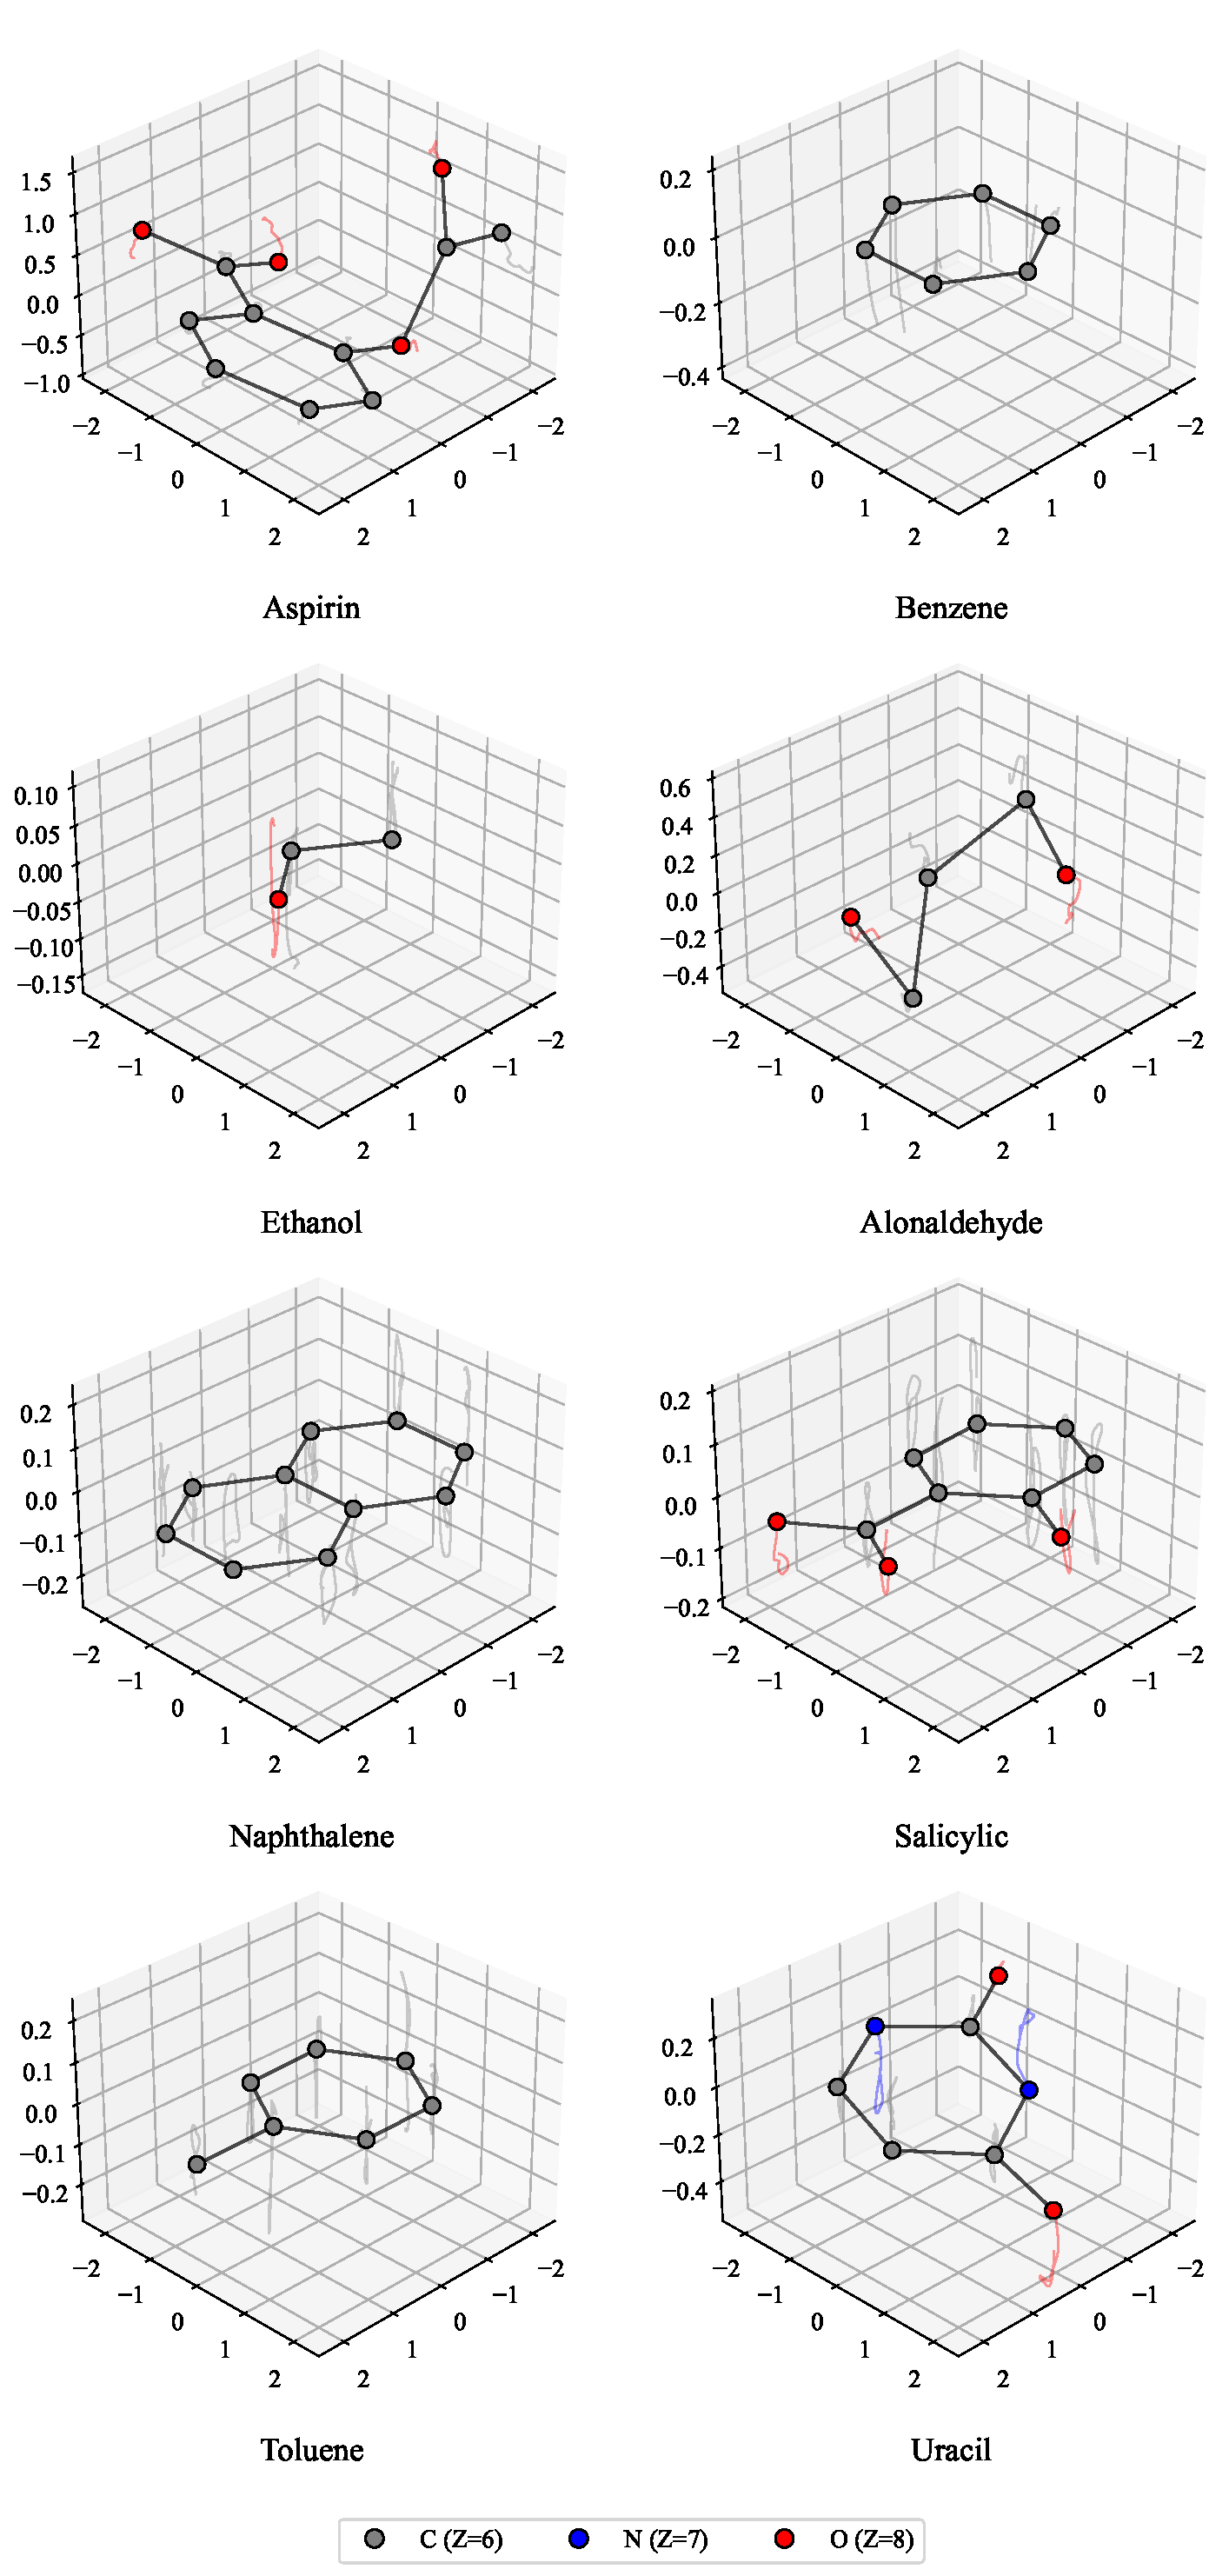
\includegraphics[width=\linewidth]{Figures/dataset/md17_combined_trajectories.pdf}
        \caption{MD17 trajectories}
        \label{fig:MD17_trajectories}
    \end{subfigure}
    \hfill
    \begin{subfigure}{0.48\linewidth}
        \centering
        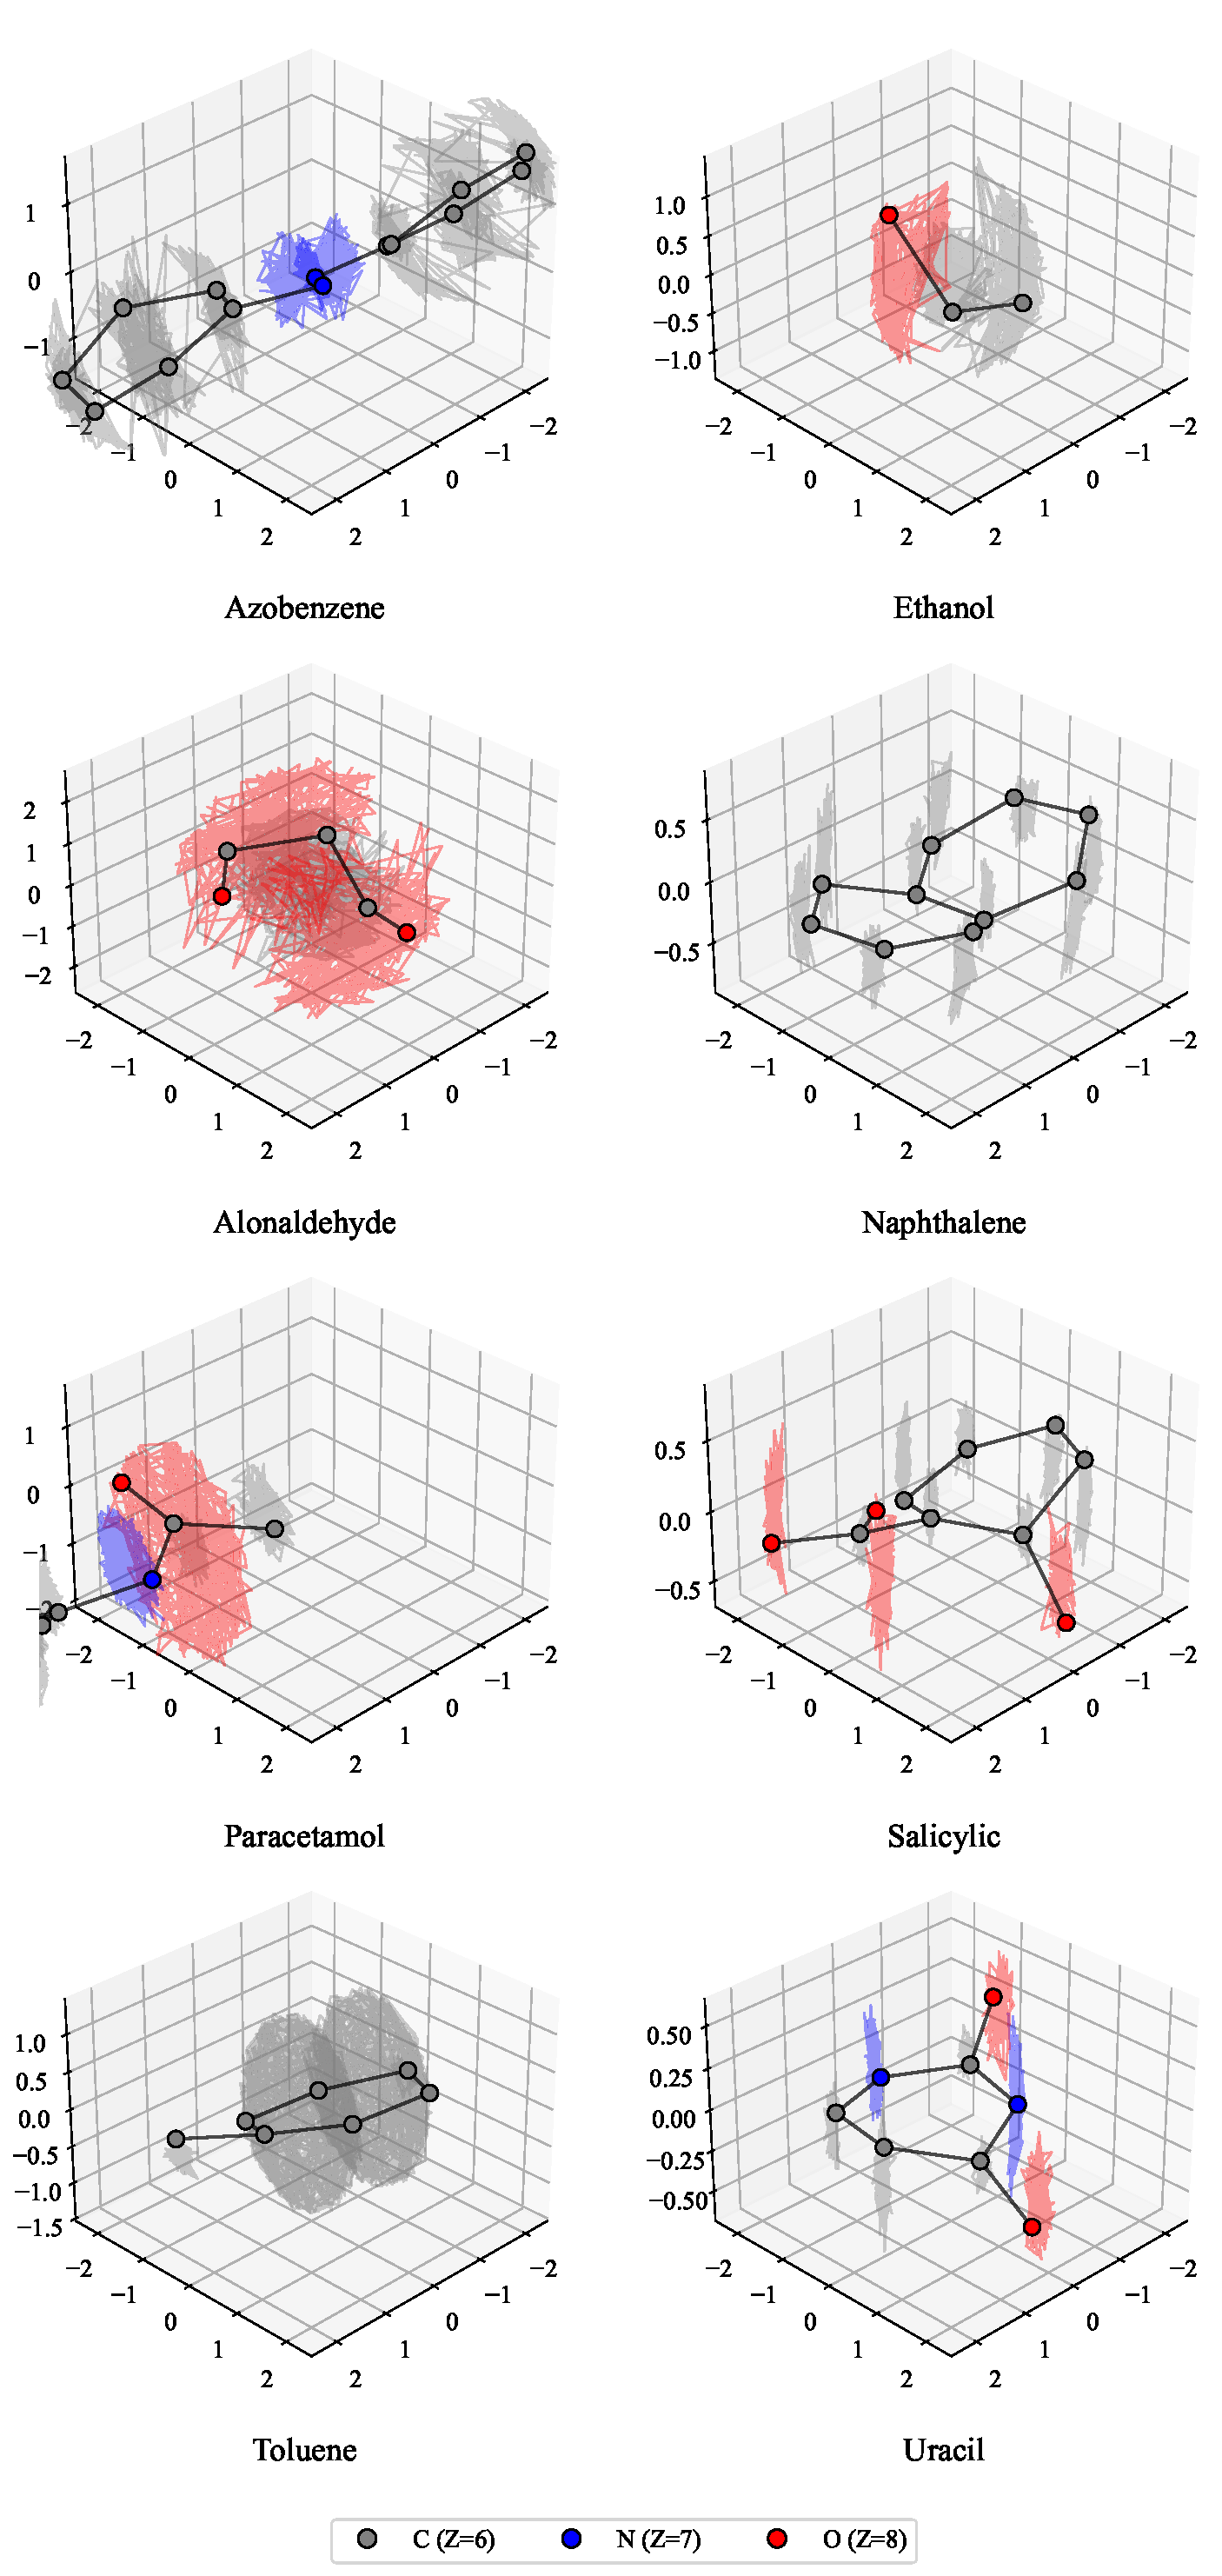
\includegraphics[width=\linewidth]{Figures/dataset/rmd17_combined_trajectories.pdf}
        \caption{RMD17 trajectories}
        \label{fig:RMD17_trajectories}
    \end{subfigure}
    \caption{3000 steps \gls{md} trajectories from the MD17 and RMD17 datasets.}
    \label{fig:trajectories}
\end{figure}
\newpage
\begin{figure}[H]
    \centering
    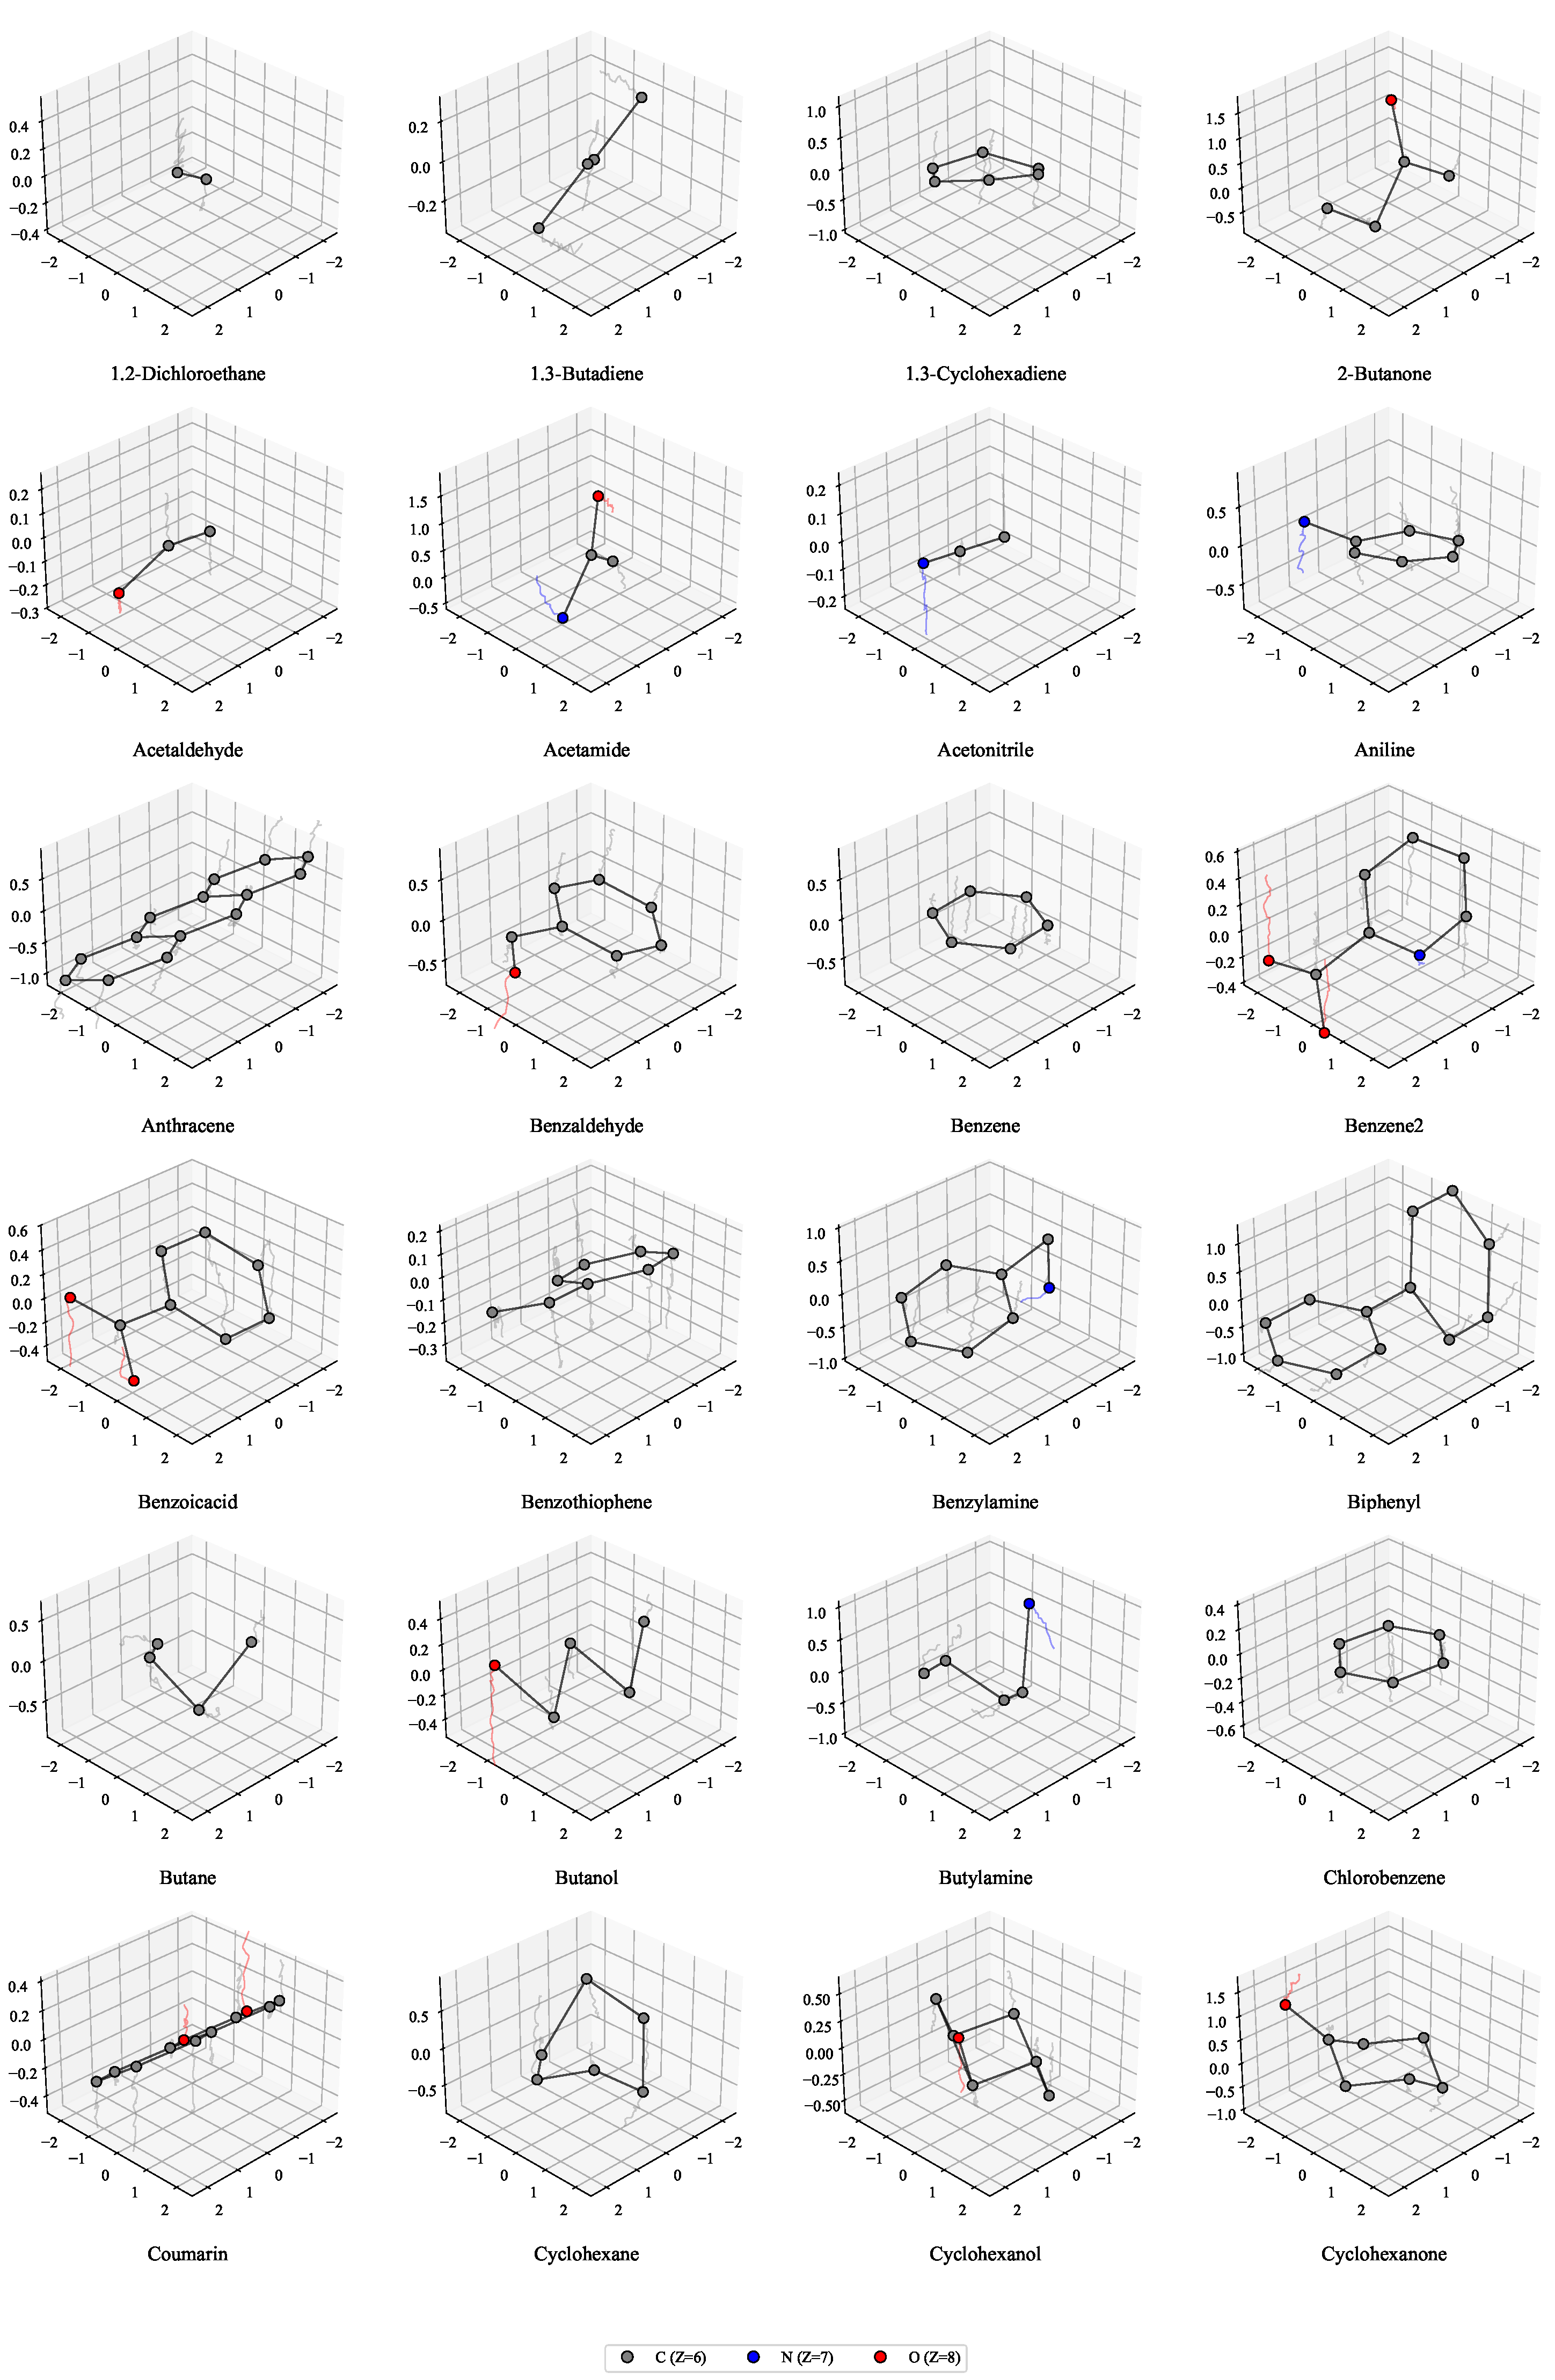
\includegraphics[width=\linewidth]{Figures/dataset/tg80_combined_trajectories_1.pdf}
    \label{fig:TG80_trajectories_1}
\end{figure}
\begin{figure}
    \centering
    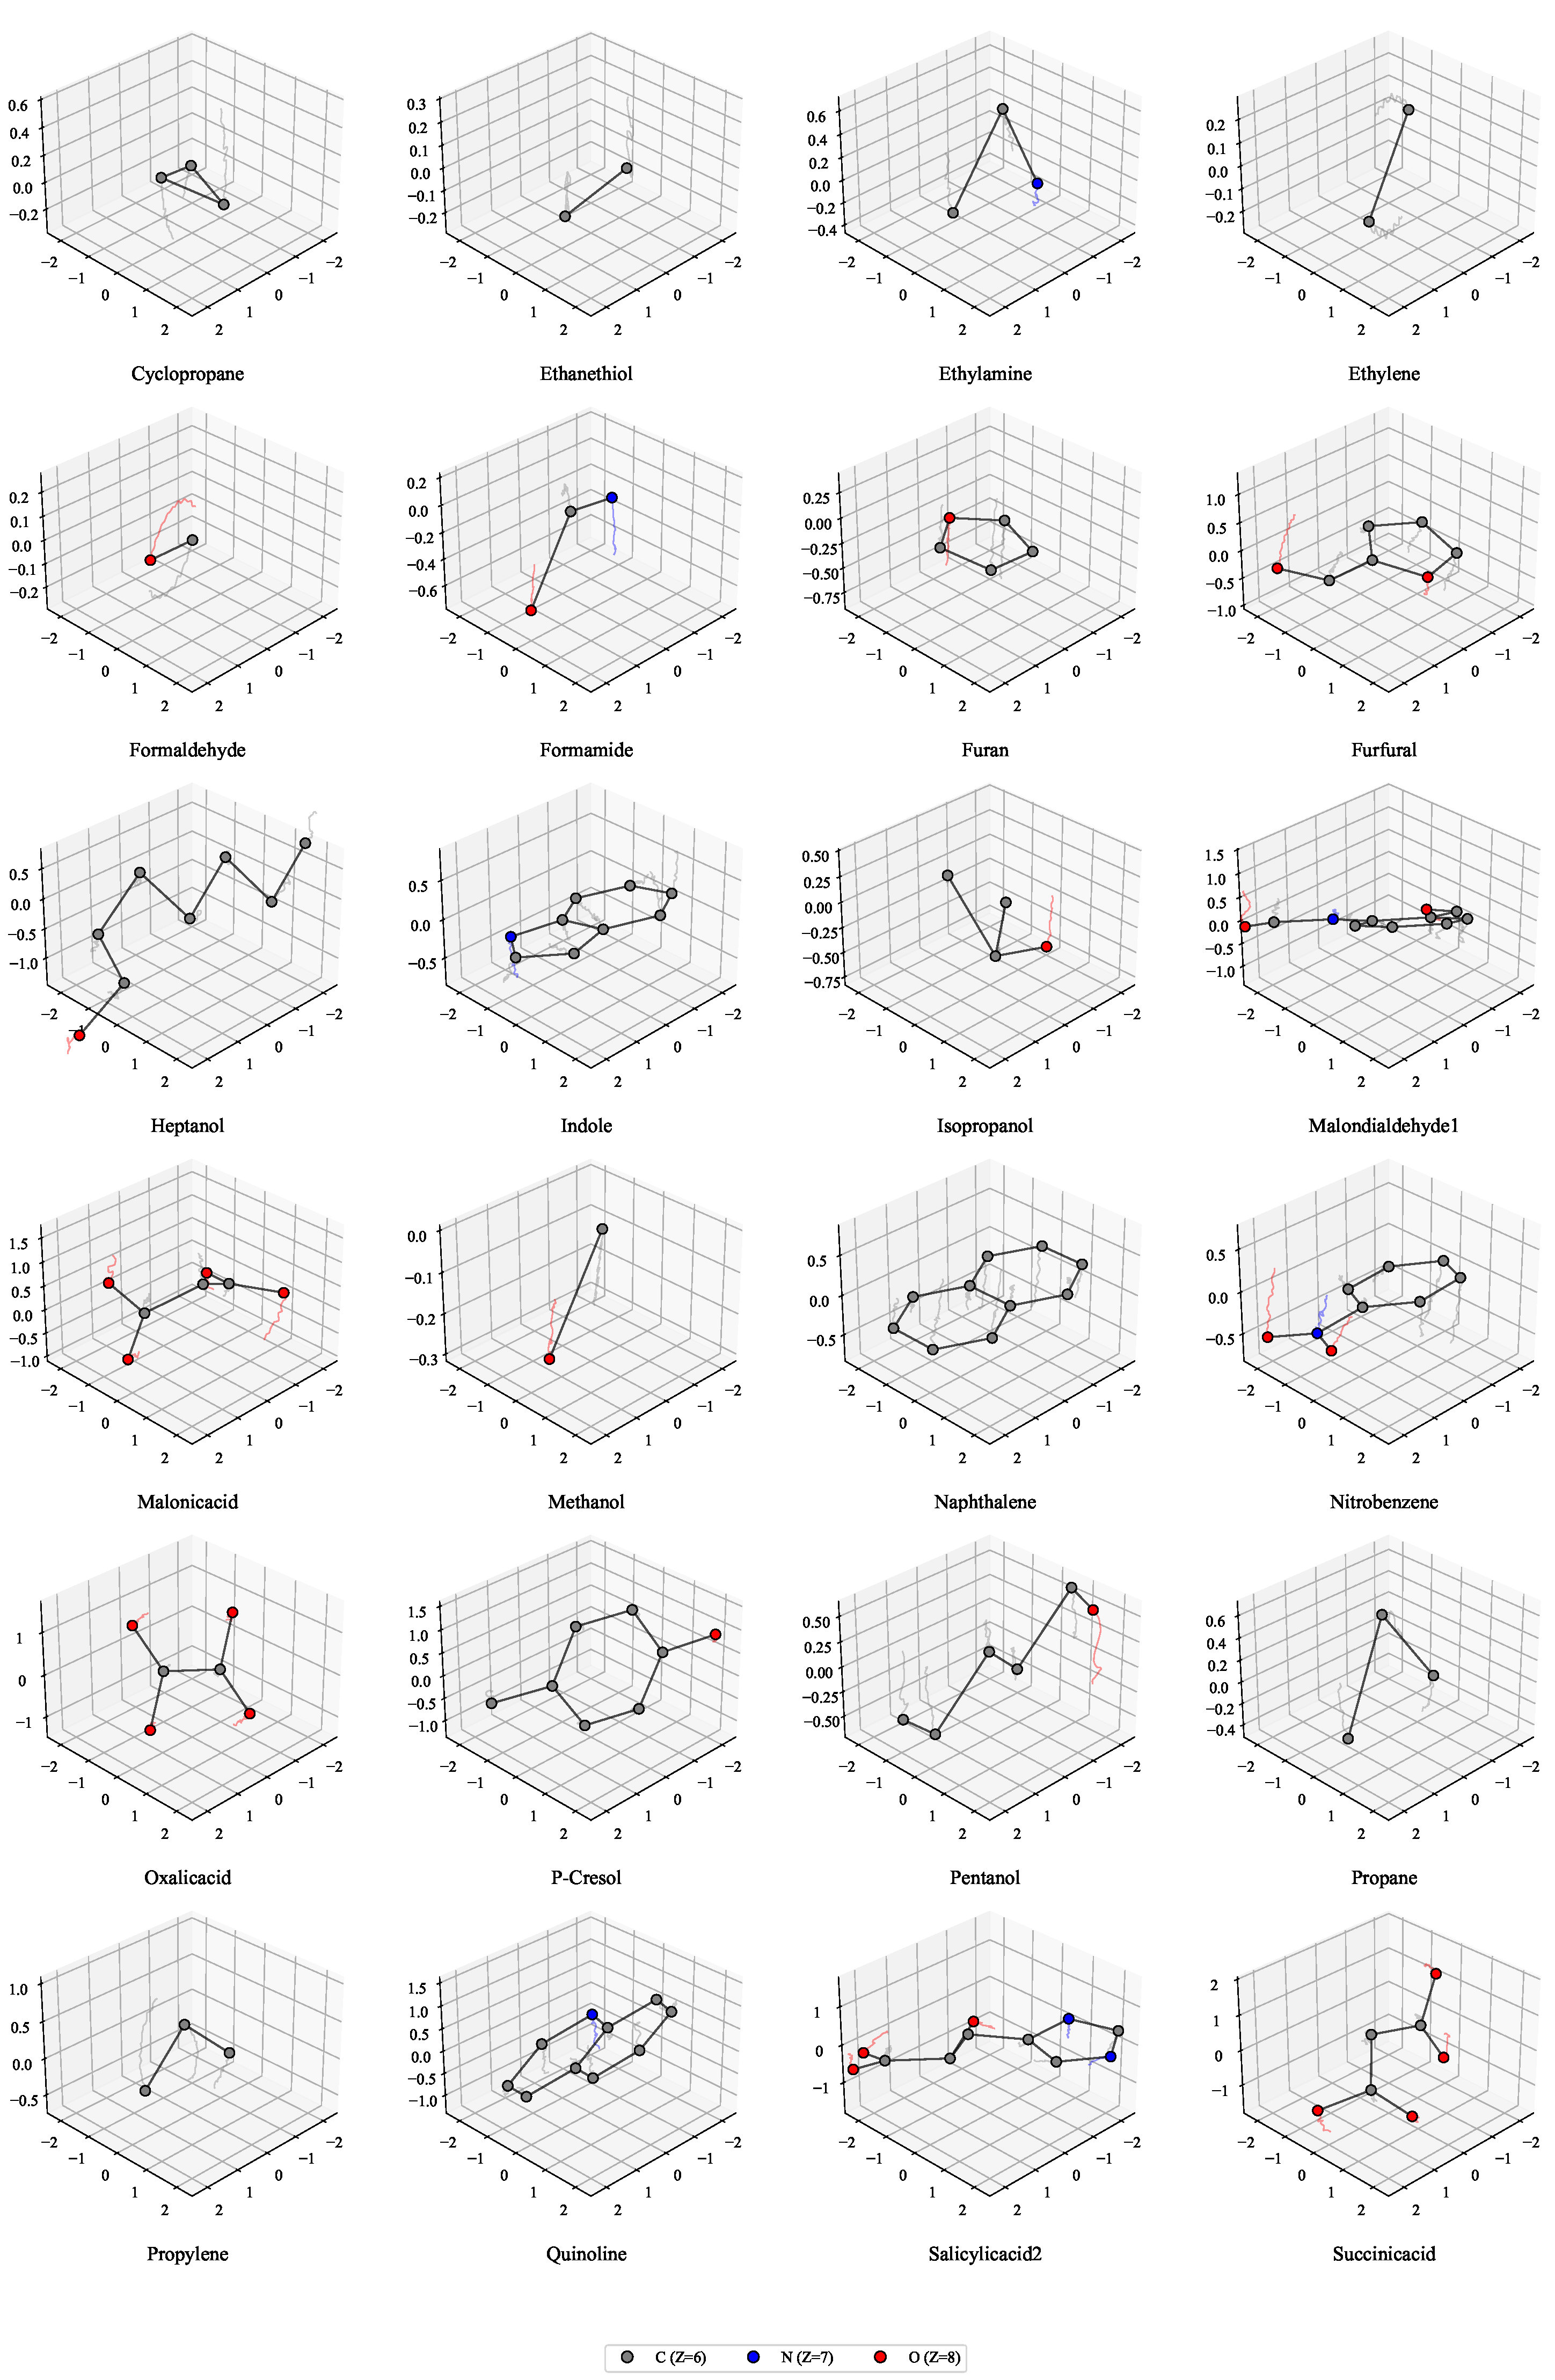
\includegraphics[width=\linewidth]{Figures/dataset/tg80_combined_trajectories_2.pdf}
    \label{fig:TG80_trajectories_2}
\end{figure}
\begin{figure}
    \centering
    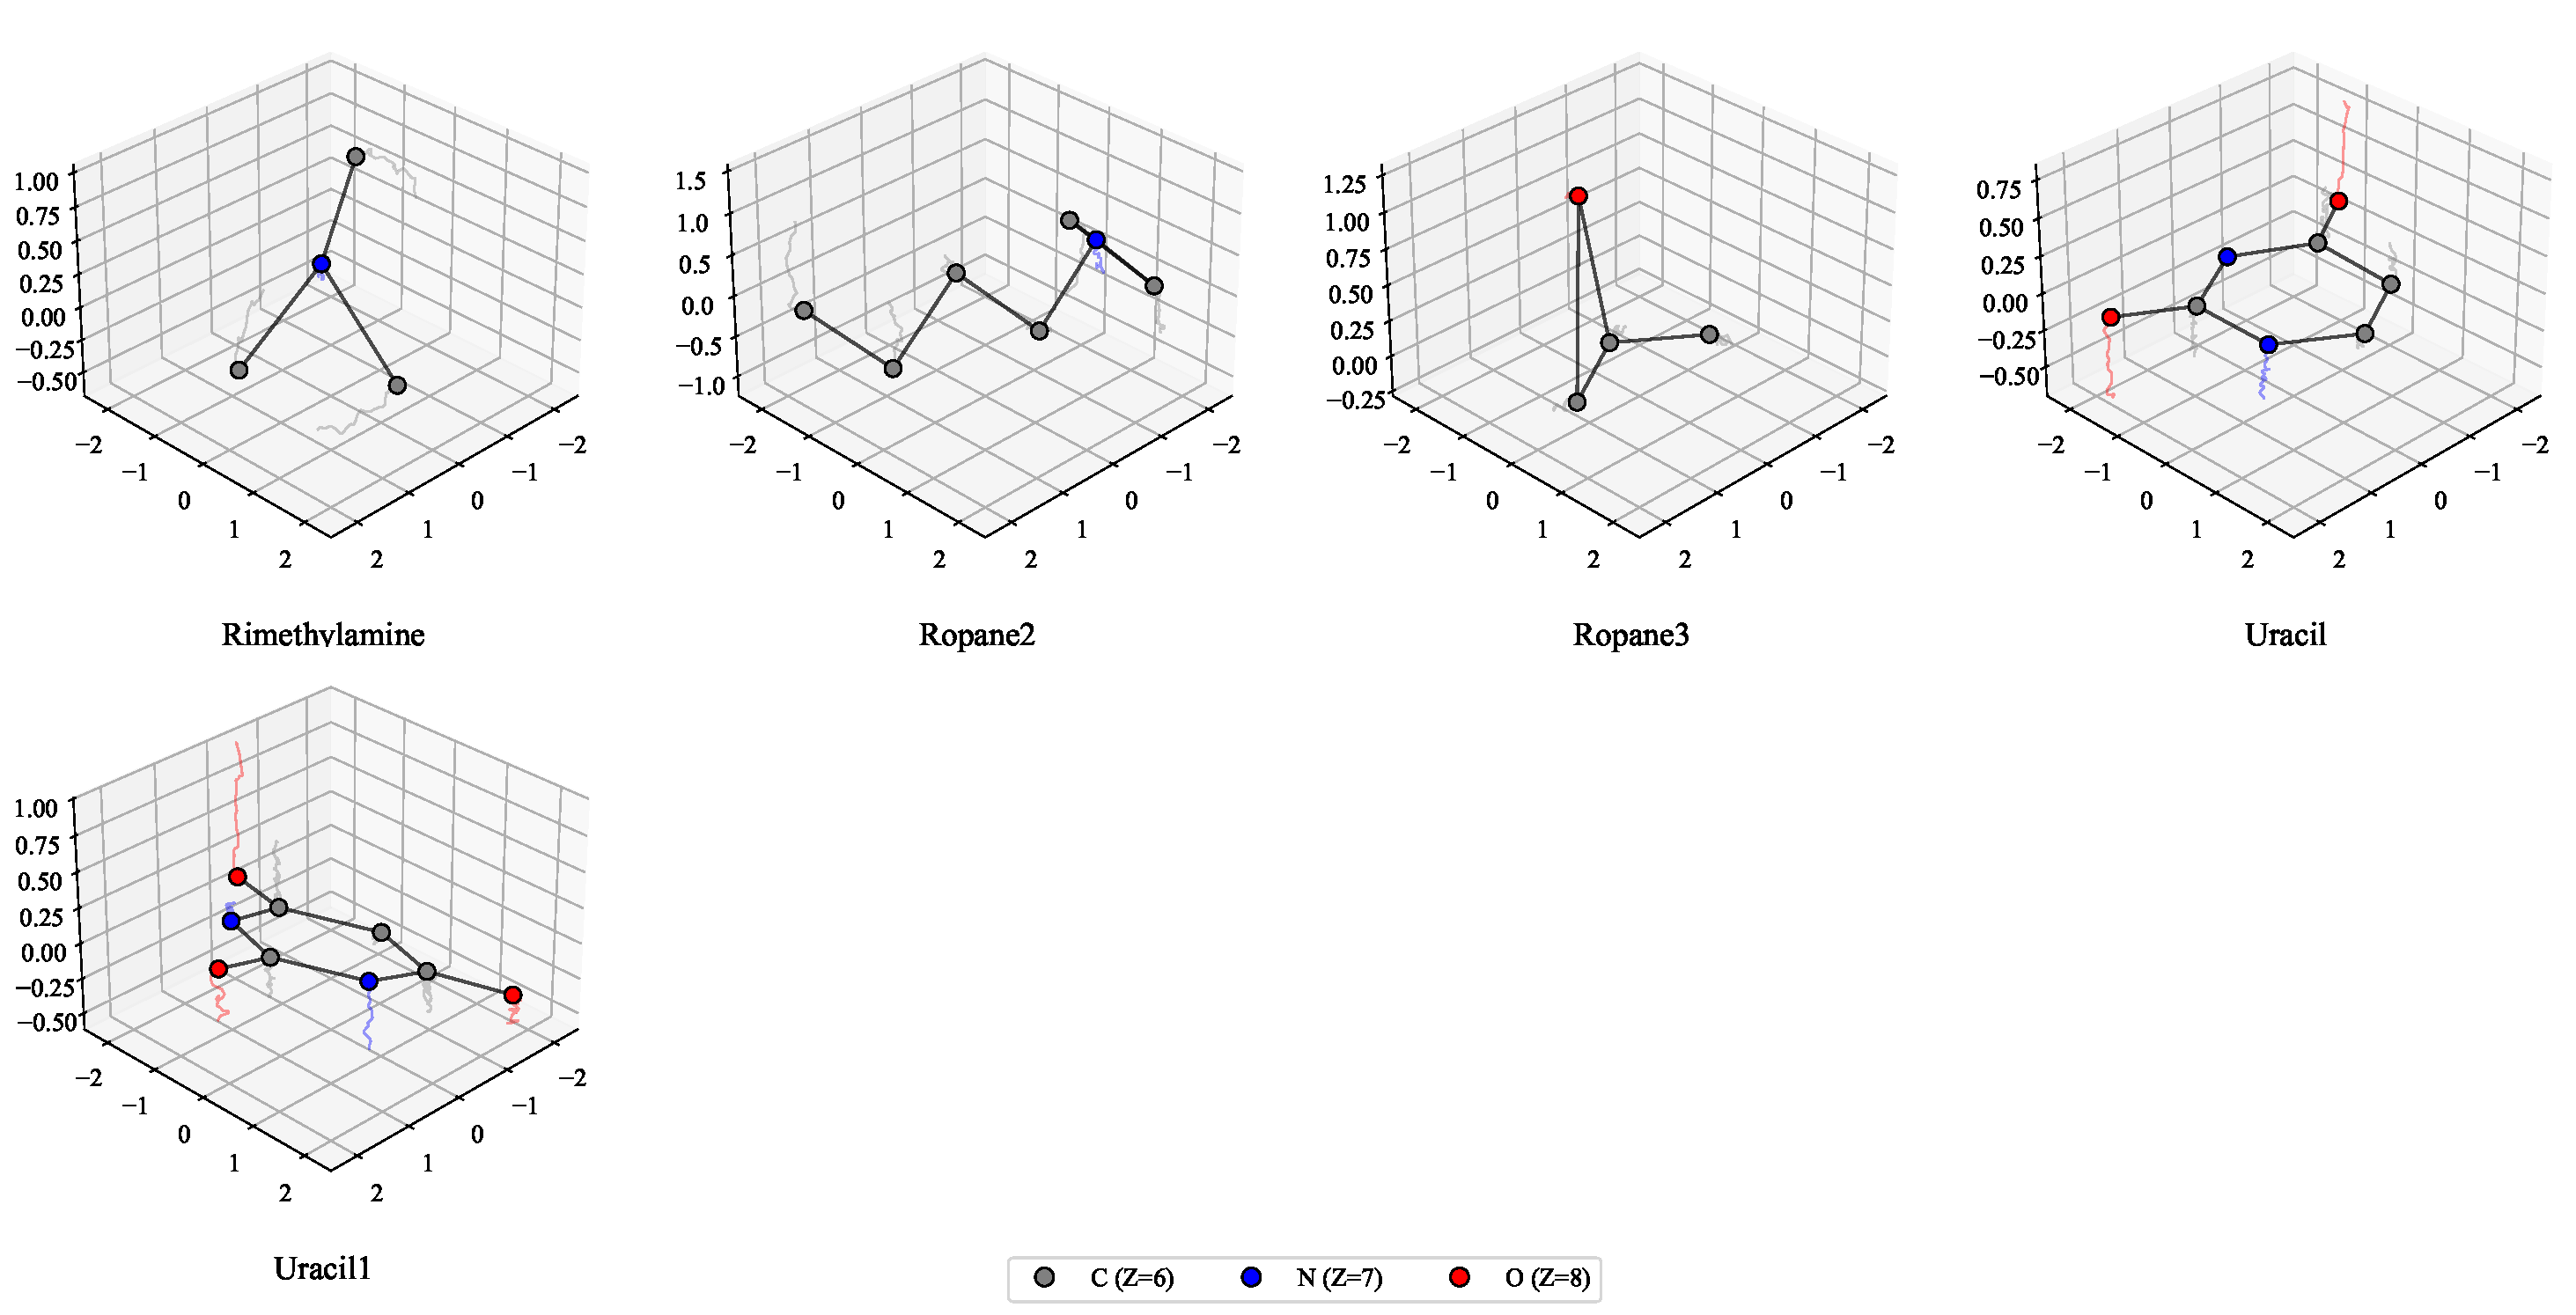
\includegraphics[width=\linewidth]{Figures/dataset/tg80_combined_trajectories_3.pdf}
    \label{fig:TG80_trajectories_3}
    \caption{3000-step \gls{md} trajectories from TG80. Molecules generated by our dataset expansion algorithm are named according to their seed molecule and the order of their selection.}
\end{figure}


